\documentclass[10pt,twoside,titlepage]{article}
\usepackage{amsmath}
\usepackage{amssymb}
\usepackage{amsfonts}
\usepackage[pdftex]{graphicx}
\usepackage{caption}
\usepackage{subcaption}
\usepackage{fancyhdr}
\setlength{\headheight}{24pt}
\usepackage[inner=3cm,outer=2cm]{geometry}
\pagestyle{fancy}
\bibliographystyle{plain}

\linespread{1.4}
\usepackage{parskip}
\setlength{\parindent}{15pt}

\newtheorem{theorem}{Theorem}[section]

\newcommand{\bx}{\mathbf{x}}
\newcommand{\by}{\mathbf{y}}
\newcommand{\bX}{\mathbf{X}}
\newcommand{\bY}{\mathbf{Y}}
\newcommand{\real}{\mathbb{R}}
\newcommand{\sysIIN}{\mbox{$I \overset{N}{\rightarrow} I$}}
\newcommand{\sysII}{\mbox{$I \rightarrow I$}}
\newcommand{\sysIJN}{\mbox{$I \overset{N}{\rightarrow} J$}}
\newcommand{\sysIJ}{\mbox{$I \rightarrow J$}}
\newcommand{\sysJJN}{\mbox{$J \overset{N}{\rightarrow} J$}}
\newcommand{\sysJJ}{\mbox{$J \rightarrow J$}}

\DeclareMathOperator*{\argmin}{arg\,min}

\begin{document}
\title{Two-Source Channel Optimized Quantization}
\author{Students: Jamie MacDonald, Peter Thompson  \\ Supervisors: Dr. Fadi Alajaji, Dr. Tamas Linder}
\maketitle


\section{Acknowledgments}
We would like to thank Professors Alajaji and Professor Linder for all their support and encouragement over the course of this project.

\begin{abstract}
In this study, a network communication system involving two transmitters and a single receiver is investigated. In particular, the impact of using a joint decoder system with channel optimized vector quantization is explored. New theory and techniques are developed, building in part on conditions of optimality for vector quantization and channel optimized vector quantization, and Lloyd's Algorithm and the Linde-Buzo-Gray Algorithm. We explore the application of this communication system to stereoscopic images and correlated bivariate Gaussian data. The implementation of the system introduces some new design challenges, which require adaption of previous quantizer algorithms, and a new pre-quantization step. Significant performance gains over independent encoders are shown  for high correlation using Gaussian data. Improvements to the system that could further enhance performance are discussed.
\end{abstract}

\tableofcontents

\section{Introduction}
Communication systems play an important role in our lives. Many communication systems operate wirelessly and are used in a variety of applications ranging from deep-space communication to cellular networks. Communication is performed with a number of different techniques, technologies, and transmission media, each presenting their own unique design challenges. Many communication systems are affected by channel noise and such channel interference can impact the data as it is being transmitted. This can lead to incorrect decoding at the receiver. Encoding schemes are used to protect data against channel interference. This is known as \emph{channel coding}. At the same time, it is also desirable to minimize channel use when communicating in order to save power and bandwidth. Data can be compressed before it is transmitted over the channel to make the best use of channel resources and to save on power. Compressing data in this way is known as \emph{source coding}. Source and channel coding typically involved transforming the data in some way. The receiver is responsible for decoding the message by inverting the transformation to recover the data.

There are a number of different ways of encoding and decoding data. Quantization is a method which involves mapping values from a large input set onto a smaller, typically finite set. Quantization is performed by a \emph{quantizer}. When quantization is used in a communication system, a quantizer first quantizes the data and maps it onto a corresponding index which is then transmitted as a waveform to the receiver. The receiver decodes the waveform back to an index, which is used to estimate the original data. Quantization is a form of lossy compression, which means the original data cannot be recovered exactly after it has been quantized.

The mapping of the encoding data onto the waveform is called modulation can involve shifting of the waveform into a particular frequency bandwidth, and can involve techniques like amplitude and frequency modulation. Communication systems can also either be analog or digital.

A schematic showing a general point-to-point communication system is provided in Figure~\ref{fig:comm_sys}.

\begin{figure}
        \centering
        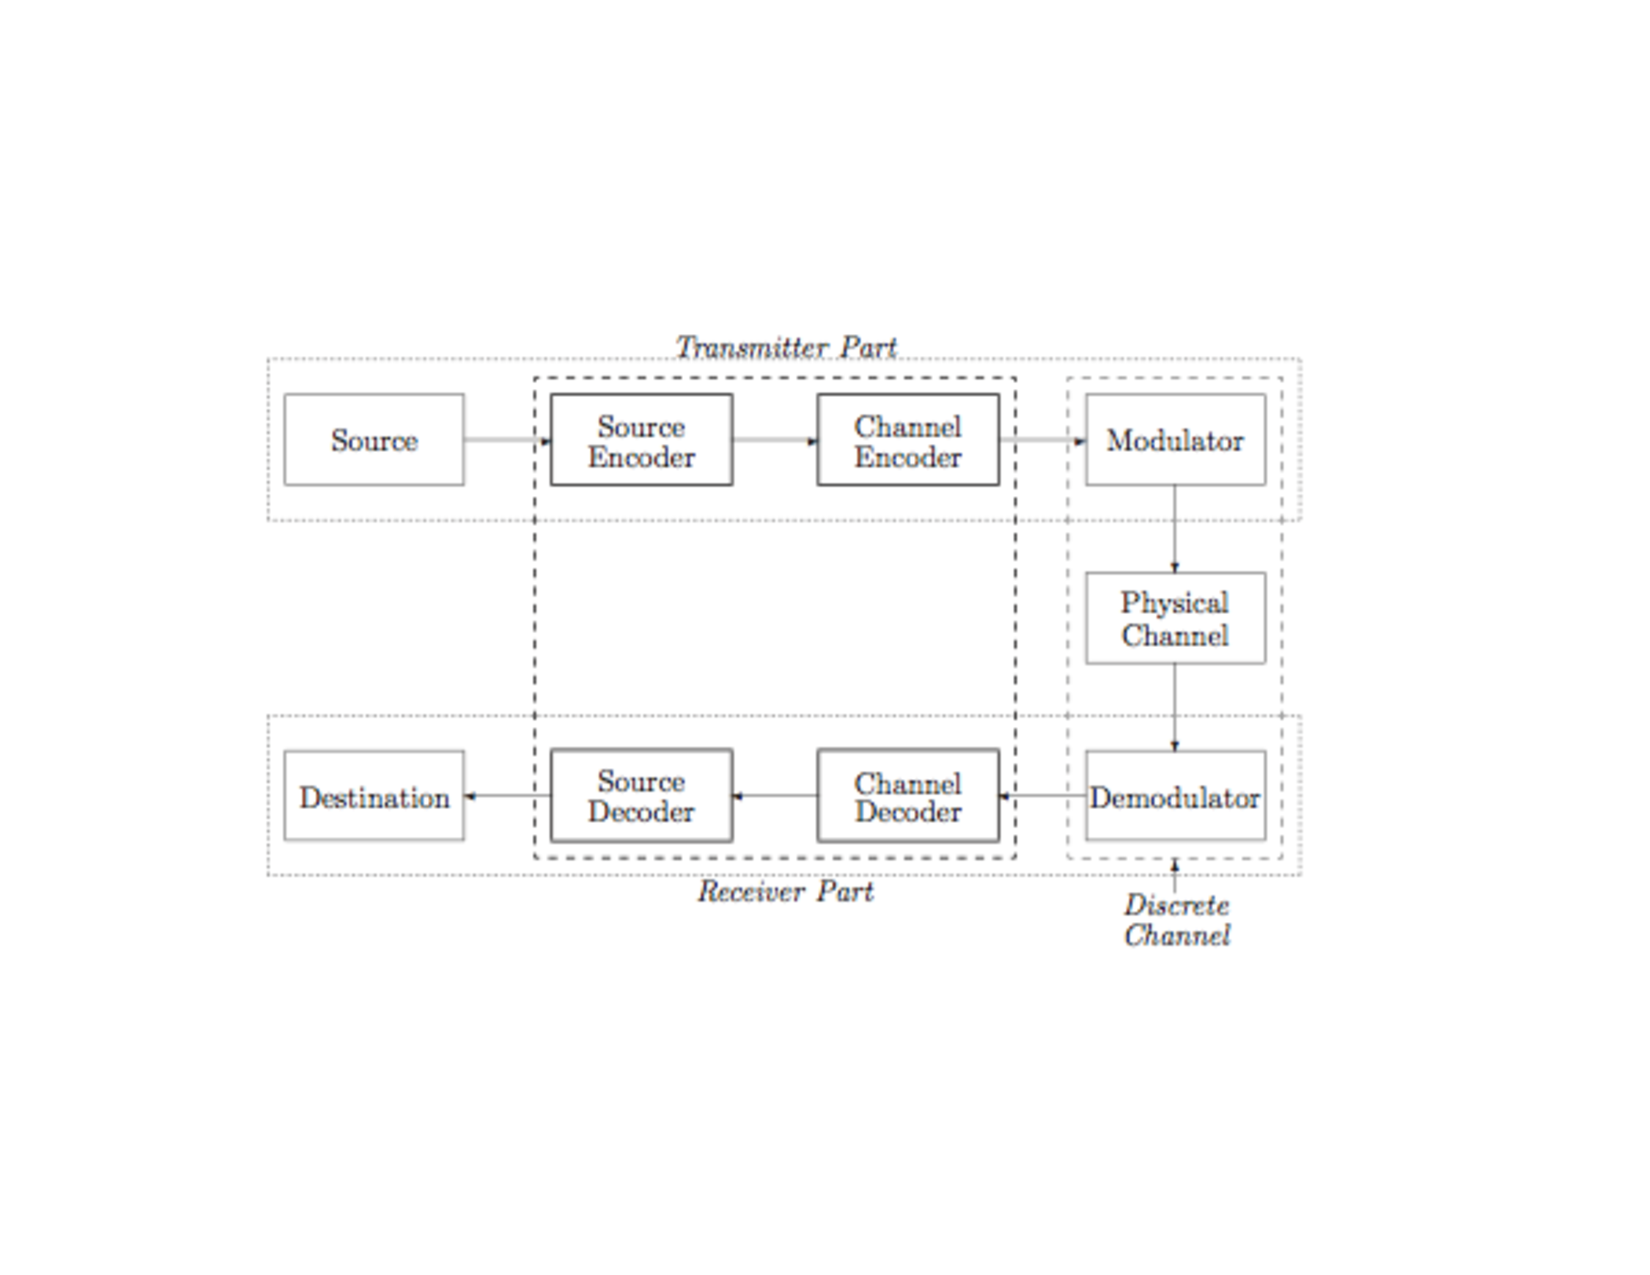
\includegraphics[width=1.1\linewidth]{comm_sys.pdf}
    \caption{An schematic of a general communication system taken from \cite{472_notes}.}
    \label{fig:comm_sys}
\end{figure}

Many applications involve more than just a single transmitter and receiver. A broadcast channel, for example, consists of a single transmitter and multiple receivers. A multiple access channel on the other hand, consists of multiple transmitters and a single receiver. A general network can consist of an arbitrary number of transmitters and receivers.

This report will focus on a network communication problem involving two transmitters and a single receiver where the data presented at the two transmitters are dependent. It will be assumed that the encoding at the two transmitters is done independently. This may correspond to the encoders being geographically separated, for example, or some other physical or technical constraint which forces them to operate independently. However, the receiver may use data dependence when decoding the two data sources.

The performance of the system will be investigated by comparing it against a similar system that uses two independent decoders at the receiver that ignore source dependence, instead of a joint decoder. The system will also be compared to a system where the two encoders are able to jointly encoder the indices before transmission. The performance of these different systems will be measured for noisy and noiseless channels. 

The performance and practical application of this joint decoder system will be explored using images. In particular, it will be assumed that the two transmitters send two dependent images, such as images of the same object. The decoder will be responsible for reconstructing the images. Special techniques for dealing with images will be dealt with in this report. Image communication techniques have had a large impact on society in recent years. Figure~\ref{fig:mars} shows an image of Martian rocks. The high similarity between the two images may imply that they can benefit from a joint decoder scheme if they are quantized.

\begin{figure}
    \centering
    \begin{subfigure}{0.5\textwidth}
        \centering
        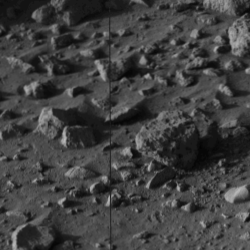
\includegraphics[width=0.6\linewidth]{mars_left.png}
        \caption{left}
    \end{subfigure}% <- this percent sign is important 8)
    \begin{subfigure}{0.5\textwidth}
        \centering
        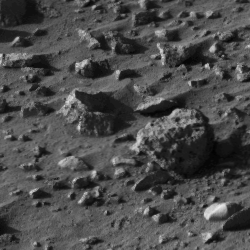
\includegraphics[width=0.6\linewidth]{mars_right.png}
        \caption{right}
    \end{subfigure}
    \caption{An example of two similar images taken on the surface of Mars.}
    \label{fig:mars}
\end{figure}

The structure of the report is as follows. Background material related to the project is presented in Section~\ref{sec:background}. A formal problem statement, and some relevant theoretical results, are  given in Section~\ref{sec:prob_desc}. Design and implementation is discussed in Section~\ref{sec:design}, and results are presented in Section~\ref{sec:results}. The results are then summarized and discussed, including suggestions of areas for future study.

\section{Background}
\label{sec:background}
Scalar and vector quantization with conditions of optimality are introduced in Section~\ref{sec:quantization}. In Section~\ref{sec:channel_optimized}, quantizers used for transmission of information over noisy channels are discussed. In Section~\ref{sec:quant_design_algos}, it is shown how conditions of optimality can be used in quantizer design. In Section~\ref{sec:code_assign}, proper codeword assignment for transmission over noisy channels is discussed. Finally, bit allocation and transform coding techniques are covered in Section~\ref{sec:bit_alloc} with a focus on images. Following the introduction of the above framework, a formal problem description and results are covered in Section~\ref{sec:design}.

\subsection{Quantization}
\label{sec:quantization}
Quantization is the process of mapping data from some large set onto a smaller, finite set. Quantization is a form of \emph{lossy compression}, which means the data can not be exactly recovered following quantization.

A quantizer with $N$ distinct output levels is called an $N$-level quantizer. The output levels of an $N$-level quantizer can be indexed from $1$ to $N$. The \emph{encoder} is a mapping which maps a point from the input space $\mathcal{S}$ onto one of these indices. The encoder mapping is denoted by $\mathcal{E}$ and can be expressed as
\begin{equation*}
\mathcal{E} : \mathcal{S} \rightarrow \{1,\ldots,N\}
\end{equation*}
The \emph{encoding region} $R_i$ is the set of points in $\mathcal{S}$ that the encoder maps onto index $i$:
\begin{equation*}
R_i = \{x \in \mathcal{S} : \mathcal{E}(x) = i\}
\end{equation*}

The encoding regions partition $\mathcal{S}$ and uniquely define $\mathcal{E}$.

Each encoder index has an associated point in $\mathcal{S}$ that is used to represent the original value of the data source. These points are called \emph{code vectors}. The set of code vectors is called the \emph{codebook} and is denoted by $\mathcal{C}$. $x_i$ is used to denote the code vector associated with index $i \in \{1,\ldots,N\}$.

Any $N$-level quantizer can be defined by the encoder-codebook pair $(\mathcal{E}, \mathcal{C})$. Moreover, the quantizer mapping $Q : \mathcal{S} \rightarrow \mathcal{S}$ is given by
\begin{equation*}
Q(x) = x_{\mathcal{E}(x)}
\end{equation*}

A distortion measure $d(x,y) : \mathcal{S}^2 \rightarrow \mathbb{R}^+$ is used to measure the performance of the quantizer. The average distortion $D_{avg}$ for a random i.i.d. source $X$, distortion measure $d(x,y)$, and quantizer $Q$, is given by
\begin{equation}
  \label{eq:D_avg}
D_{avg} = E[d(X,Q(X))]
\end{equation}
where $E$ denotes expectation.

An $N$-level quantizer is \emph{optimal} if its average distortion is less than or equal to the average distortion of all other $N$-level quantizer. In general, finding an optimal quantizer is very difficult. For example, there may be quantizers that are locally optimal, but not globally optimal.

For the rest of the report, it is be assumed that the input space $\mathcal{S}=\mathbb{R}^k$. A quantizer with $k=1$ is called a \emph{scalar quantizer}, and a quantizer with $k \ge 1$ is called a \emph{vector quantizer}. \emph{Squared-error distortion}, denoted by ${\bf {\| x - y \|}}^2$, is the distortion measure used in this report to measure quantizer performance. Squared-error distortion is defined as follows:
\begin{equation*}
{\| \bx - \by \|}^2 = \sum_{i=1}^n{(x_i - y_i)}^2
\end{equation*}
where $x_i$ and $y_i$ are the $i$th elements of $\bx$ and $\by$.

Two conditions of optimality for quantizers are now discussed. Their application to quantizer design will be presented in Section~\ref{sec:quant_design_algos}. It should be mentioned that the following conditions of optimality can be derived for more general distortion measures and input spaces. Results will only be given for squared-error distortion over $\mathbb{R}^k$ in this report. Conditions of optimality will be given for other quantizer schemes in following sections.

The first condition of optimality is the \emph{centroid condition}. The centroid condition states that each code vector should be placed at the centroid of its corresponding encoding region. A more formal statement is as follows:

\begin{theorem}
\label{theo:cent_vq}
Amongst the set of all $N$-level quantizers with encoding function $\mathcal{E}$, the quantizer with code vectors
\begin{align}
  \label{eq:cent_vq}
  \bx_i &= E[\bX | \bX \in R_i] \\
&= \frac{ \int_{R_i}\bx f(\bx)d\bx }{ \int_{R_i}f(\bx)d\bx }
\end{align}
for all $i \in \{1,\ldots,N\}$ has minimum distortion.
\end{theorem}

The second condition of optimality is the \emph{nearest neighbor condition}. The nearest neighbor condition states that the encoder mapping $\mathcal{E}$ should be chosen so each point in $\mathbb{R}^k$ maps onto the code vector of lowest distortion:

\begin{theorem}
Consider all $N$-level quantizers with codebook $\mathcal{C}$. The quantizer with encoding regions satisfying
\begin{equation*}
R_i \subset \{\bx : \| \bx - \bx_i \| \le \| \bx - \bx_j \| \text{ for all } j = 1,\ldots,N \}
\end{equation*}
for all $i \in \{1,\ldots,N\}$ has minimum distortion.
\end{theorem}

Notice that subsets are used to constrain the encoding regions. This is done to break ties between points of equal distortion between multiple code vectors. These boundary points can be mapped arbitrarily to break ties.

The centroid and nearest neighbor conditions provide necessary conditions of optimality for an optimal quantizer, but they are not sufficient. A quantizer whose encoder mapping $\mathcal{E}$ and codebook $\mathcal{C}$ satisfy the conditions of optimality is called a Lloyd-Max quantizer. Note that an optimal quantizer can be defined just by its codebook $\mathcal{C}$, because the nearest neighbor condition can be applied to determine $\mathcal{E}$.

It is possible to rewrite the average distortion $D_{avg}$ from (\ref{eq:D_avg}) for a vector quantizer as follows:
\begin{align*}
D_{avg} &= \sum_{i=1}^{N} E[ {\| \bX -  \bx_i\|}^2 | \bX \in R_i] P(\bX \in R_i) \\
&= \sum_{i=1}^{N} \int_{R_i} {\|\bx - \bx_i\|}^2 p(\bx) d\bx
\end{align*}

\subsection{Channel Optimized Quantization}
\label{sec:channel_optimized}
The use of quantization in communication systems with noisy channels is now discussed. In this scenario, the index from the encoder is transmitted over a noisy channel to the receiver, but channel interference can influence which index is received. A channel optimized quantizer is designed according to the channel and source distribution in order to minimize the distortion between the source value and estimate at the receiver. Nearest neighbor and centroid conditions still apply for a channel optimized quantizer, but they now depend on both the channel properties and source distribution, and have to be adjusted accordingly for the new system.

The channel that will be considered in this paper is assumed to be memoryless, which means the properties of the channel do not change after each channel use. To transmit an index over the channel, the index is first mapped onto a string of channel symbols of fixed length by a mapping $b$. This representation is then used to transmit the index over the channel. The receiver used the inverse mapping of $b$ to obtain the received index. The probability of receiving index $j$ given index $i$ was transmitted is $P(b(j)|b(i))$. These probabilities are called the \emph{channel transition probabilities}. The mapping $b$ should also be chosen to minimize distortion; this will be discussed in Section~\ref{sec:code_assign}.

The nearest neighbor and centroid conditions for the channel optimized quantizer are now given, beginning with the centroid condition.

\begin{theorem}
\label{theo:cent_covq}
Amongst the set of all $N$-level channel quantizers with encoding function $\mathcal{E}$, the quantizer with code vectors
\begin{equation}
  \label{eq:cent_covq}
  \bx_j = \frac{\sum_{i=1}^N E[\bX | \bX \in R_i]P(b(j)|b(i))}{\sum_{i=1}^N P( \bX \in R_i)P(b(j)|b(i))} 
\end{equation}
for all $j \in \{1,\ldots,N\}$ has minimum distortion.
\end{theorem}
This is similar to the centroid condition in Theorem~\ref{theo:cent_vq}, but the centroid now depends on both the source distribution and channel probabilities. The nearest neighbor condition for channel optimized quantization is now provided.

\begin{theorem}
Consider all $N$-level quantizers with codebook $\mathcal{C}$. The quantizer with encoding regions satisfying
\begin{equation*}
R_j \subset \left\{x : \sum_{i=1}^N {\| \mathbf{x} - \mathbf{x_i} \|}^2P(j|(i)) \le \sum_{i=1}^N {\| \mathbf{x} - \mathbf{x_i} \|}^2P(b(k)|b(i)) \text{ for all } k = 1,\ldots,N \right\}
\end{equation*}
for all $j \in \{1,\ldots,N\}$ has minimum distortion.
\end{theorem}

The average distortion for an $N$-level channel quantizer is
\begin{align}
  \label{eq:channel_dist}
D_{avg} &= \sum_{i=1}^{N} \sum_{j=1}^{N} E[ {\|\bX - \bx_j\|}^2 | \bX \in R_i] P(\bX \in R_i) P(b(j)|b(i))\\
&= \sum_{i=1}^{N} \sum_{j=1}^{N} P(b(j)|b(i)) \int_{R_i} {\|\bx - \bx_j\|}^2 f(\bx) d\bx
\end{align}

One practical advantage of using channel optimized quantization  is that it performs source and channel coding in a single step. This means it is able to compress the incoming data while encoding it so it is resilient to channel interference at the same time. Performing source and channel coding jointly, rather than in tandem, is beneficial because it can be more computationally efficient.

\subsection{Quantizer Design Algorithms}
\label{sec:quant_design_algos}
The Lloyd-Max and Linde-Buzo-Gray quantizer design algorithms are now discussed. These two algorithms rely on the previously discuses conditions of optimality. A big advantage of these algorithms is that they do not require the underlying source distribution, and can instead be used to design a quantizer using a training set taken from the source distribution. Recall that an optimal quantizer can be defined by its codebook, since the encoder can be obtained from the codebook by applying the nearest neighbor condition, so only the globally optimal codebook needs to be considered.

The Lloyd-Max algorithm is now discussed. Recall that the nearest neighbor condition optimizes the encoder for a fixed codebook, and the centroid condition optimizes the codebook for a fixed encoder. The Lloyd-Max algorithm iteratively applies the centroid and nearest neighbor conditions using training set until the codebook converges. The Lloyd-Max algorithm is implemented using a training set $\mathcal{T}$ taken from the source distribution. An overview of the algorithm follows:

\medskip

{\noindent \sc Lloyd-Max Algorithm}
\begin{enumerate}
\item Start with the codebook in some initial state.
\item Apply the nearest neighbor condition to each point in $\mathcal{T}$. Let $R(i) \subset \mathcal{T}$ denote the set of points that map onto index $i$.
\item Move each code vector $\bx_i$ to the centroid of $R(i)$ by applying the centroid condition.
\item Return to step (2). Finish once the training set distortion has converged.
\end{enumerate}

One limitation of the Lloyd-Max algorithm is that is does not guarantee convergence to an optimal quantizer. The performance of the quantizer is dependent on the initial state of the codebook before starting the algorithm. It is important that the codebook is initialized properly to ensure convergence onto a good codebook.

The Linde-Buzo-Gray can be used in conjunction with the Lloyd-Max algorithm to improve initialization conditions to obtain a better codebook. In the LBG algorithm, the codebook initially contains a single code vector placed at the centroid of the entire training set. Code vectors are iteratively split in two in between iterations of the Lloyd-Max algorithm until the final codebook size is obtained. A more detailed description of the algorithm follows:

\medskip

{\sc \noindent Linde-Buzo-Gray Algorithm}
\begin{enumerate}
\item Begin with an initial codebook $\mathcal{C}$ containing a single code vector placed at the centroid of the training set $\mathcal{T}$.
\item Let $N$ denote the size of the codebook $\mathcal{C}$ with code vectors denoted by $\bx_i$ for $i \in \{1,\ldots,N\}$. Construct a new codebook $\mathcal{C}^*$ of size $2N$ with code vectors $x_i^* = (1-\epsilon)x_i$, $x_{i+N}^* = (1+\epsilon)x_i$ for all $1 \le i \le N$ and some small $\epsilon$.
\item Let $\mathcal{C}=\mathcal{C}^*$
\item Apply the Lloyd-Max algorithm to $\mathcal{C}$.
\item Return to step (2). Finish once the desired codebook size has been reached
\end{enumerate}

The LBG algorithm can provide better initialization conditions than if an arbitrary initial codebook was used and can therefore results in a better quantizer. Convergence onto an optimal solution is still not guaranteed using the LBG algorithm, however.

Other methods of improving quantizer performance are discussed in the remaining two subsections.

\subsection{Binary Codeword Assignment}
\label{sec:code_assign}
In channel optimized quantization it is important that the index mapping $b$ is chosen appropriately in order to minimize distortion. Recalling the equation for average distortion for the noisy channel in (\ref{eq:channel_dist}), it was shown in \cite{favardin} that if the codebook satisfies the centroid condition, the average distortion can be expressed as
\begin{equation}
\label{eq:codeword_distortion}
D_{avg}  = \sum_{i=1}^N \int_{R_i} {\|\bx - \bx_i\|}^2p(\bx)d\bx + \sum_{i=1}^N \sum_{j=1}^N P(\bX \in R_i) P(b(j)|b(i)) {\|\bx_i - \bx_j\|}^2
\end{equation}

Only the second term on the right-hand side is dependent on the mapping $b$. Therefore, it is possible to minimize the average distortion in $b$ for a fixed encoder and codebook by considering only this term.

One interpretation of (\ref{eq:codeword_distortion}) is that the first term on the right-hand side quantifies the distortion by quantization onto $x_i$, and the second term corresponds to the distortion due to transmitting the index over the channel. The second term will be denoted by $D_C$ and is given by
\begin{equation}
  \label{eq:codeword_dist}
D_C = \sum_{i=1}^N \sum_{j=1}^N P(\mathbf{X} \in R_i) P(b(j)|b(i)) \|\mathbf{x_i} - \mathbf{x_j}\|
\end{equation}
Minimizing (\ref{eq:codeword_dist}) for a fixed codebook lies in the set of problems which are NP-complete, which means they are computationally expensive to solve. This minimization may not be practical for a large codebook, but there are a number of methods tfor obtaining a good approximation to the optimal solution. Simulated annealing will be used as pert of the implementation in this study, and will be discussed in more detail in Section~\ref{sec:sim_anneal}.

\subsection{Bit Allocation and Transform Coding}
\label{sec:bit_alloc}
Additional quantization techniques will now be discussed with application to images. Consider a block of scalars $X_1,\ldots,X_k$ that is to be quantized. Instead of applying vector quantization to the block, $k$ scalar quantizers will be used instead. One reason for doing this is that scalar quantizers can be more efficient in practice. The overall distortion of the block is
\begin{equation*}
E\left[\sum_{i=1}^k(X_i - Q(X_i))^2\right]
\end{equation*}
It is assumed that the quantized block must be constrained to $B$ bits per block:
\begin{equation*}
\sum_{i=1}^k \log_2 N_i \le B
\end{equation*}
The $k$ scalar quantizers can be designed using the previously mentioned algorithms, but the bits now need to be allocated amongst the quantizers such that the total distortion is minimized. This is known as bit allocation, and optimal bit allocation can drastically reduce the block distortion.

\section{Problem Description}
\label{sec:prob_desc}
As mentioned in the Introduction, the system to be analyzed in this report consists of two transmitters that independently transmit an index over a channel to a single receiver. The receiver uses the two received indices to estimate the two sources. It is assumed that the two sources are dependent, so a joint decoder which uses both indices to estimate each source should obtain better source estimates than if only one index was used to estimate each source. Noisy and noiseless channels will be analyzed in this report.

It is assumed that each of the two sources is scalar valued. Let $(X,Y)\in\real^2$ denote the random source which has a density function $f(x,y)$. The encoder $\mathcal{E}$ maps a pair $(x,y) \in \mathbb{R}^2$ onto a pair of indices $i$ and $j$:
\begin{equation*}
    \mathcal{E} : \real^2\to\{1,\ldots,N_X\} \times \{1,\ldots,N_Y\}
\end{equation*}
where $N_X$ and $N_Y$ are the number of output levels for the two encoders. If $X$ and $Y$ are encoded independently (as in the main system to be studied), $\mathcal{E}$ can be expressed as two separate encoders
\begin{gather*}
    \mathcal{E}_X : \real\to\{1,\ldots,N_X\} \\
    \mathcal{E}_Y : \real\to\{1,\ldots,N_Y\}
\end{gather*}
so that $\mathcal{E}(x,y) = (\mathcal{E}_X(x), \mathcal{E}_Y(y))$. If encoding is not done independently, it is said to be done jointly. Let $R_{i,j} \subset \mathbb{R}^2$ denote the encoding region associated with index $i$ and $j$. When encoding is performed independently, the encoding regions can be expressed as $R_{i,j} = R_i^X \times R_j^Y$ where $R_i^X$ is the encoding region for $\mathcal{E}_X$ and index $i$, and $R_j^Y$ is the encoding region for $\mathcal{E}_Y$ for index $j$.

Let $k$ denote the index received at the receiver corresponding to index $i$ and let $l$ denotes the index at the receiver corresponding to index $j$. The indices $k$ and $l$ are used to estimate $X$ and $Y$ by the decoder. Let 
\begin{equation}
\mathcal{C} = \{ (x_{k,l},y_{k,l}) : k = 1,\ldots,N_X, l = 1,\ldots,N_Y\}
\end{equation}
denote the codebook used to make this estimate. The code vector pair $(x_{k,l},y_{k,l})$ corresponds to the estimates of $X$ and $Y$ given indices $k$ and $l$ were received. Decoding of $X$ and $Y$ is done independently if the estimate of $X$ only depends on index $k$ and the estimate of $Y$ only depends on $l$. In this case, let
\begin{align}
\mathcal{C}_X &= \{x_k : k = 1,\ldots,N_X\} \\
\mathcal{C}_Y &= \{y_l : l = 1,\ldots,N_Y\}
\end{align}
denote the codebooks for $X$ and $Y$. Note that $\mathcal{C} = \mathcal{C}_X \times \mathcal{C}_Y$ when decoding independently.

The sum of the squared-error distortion of both sources will be used to measure performance:
\begin{equation}
\label{eq:sys_dist}
    D_{avg} = E[{(X-\hat{X})}^2 + {(Y-\hat{Y})}^2]
\end{equation}
where $(\hat X, \hat Y) \in \mathcal{C}$ represent the estimates of $X$ and $Y$ at the receiver.

In this report, different combinations of joint and independent encoders and codebook, over noisy and noiseless channel will be considered. The table below shows the notation that will be used for the different combinations:

\begin{table}
\begin{center}
    \begin{tabular}{| l | l | l | l |}
    \hline
    \bf System & \bf Encoder & \bf Codebook & \bf Channel \\ \hline \hline
    \sysII & Independent & Independent & Noiseless \\ \hline
    \sysIIN & Independent & Independent & Noisy \\ \hline
    \sysIJ & Independent & Joint & Noiseless \\ \hline
    \sysIJN & Independent & Joint & Noisy \\ \hline
    \sysJJ & Joint & Joint & Noiseless \\ \hline
    \sysJJN & Joint & Joint & Noisy \\ \hline
    \end{tabular}
    \caption{Different Encoder/Codebook setups that will be studied for the 2-source system.}
\end{center}
\end{table}

% Rewrite this
As mentioned in the Introduction, the focus of this project is on the analysis and implementation of the \sysIJ\ and \sysIJN ~where encoding is done independent and a joint decoder is used. It is clear for $N_X$ and $N_Y$ fixed, any \sysII\ (\sysIIN) can be implemented using a \sysIJ\ (\sysIJN) system, and any \sysIJ\ (\sysIJN) system can be implemented using a \sysJJ\ (\sysJJN) system. Therefore, an optimal \sysII\ (\sysIIN) system can  provide a lower bound on the performance of an optimal \sysIJ\ (\sysIJN) system for similar channel characteristics for the noisy systems. Likewise, an optimal \sysJJ\ (\sysJJN) system provides an upper bound on the performance of an optimal \sysIJ\ (\sysIJN) systems with similar channel characteristics.

\begin{figure}
        \centering
        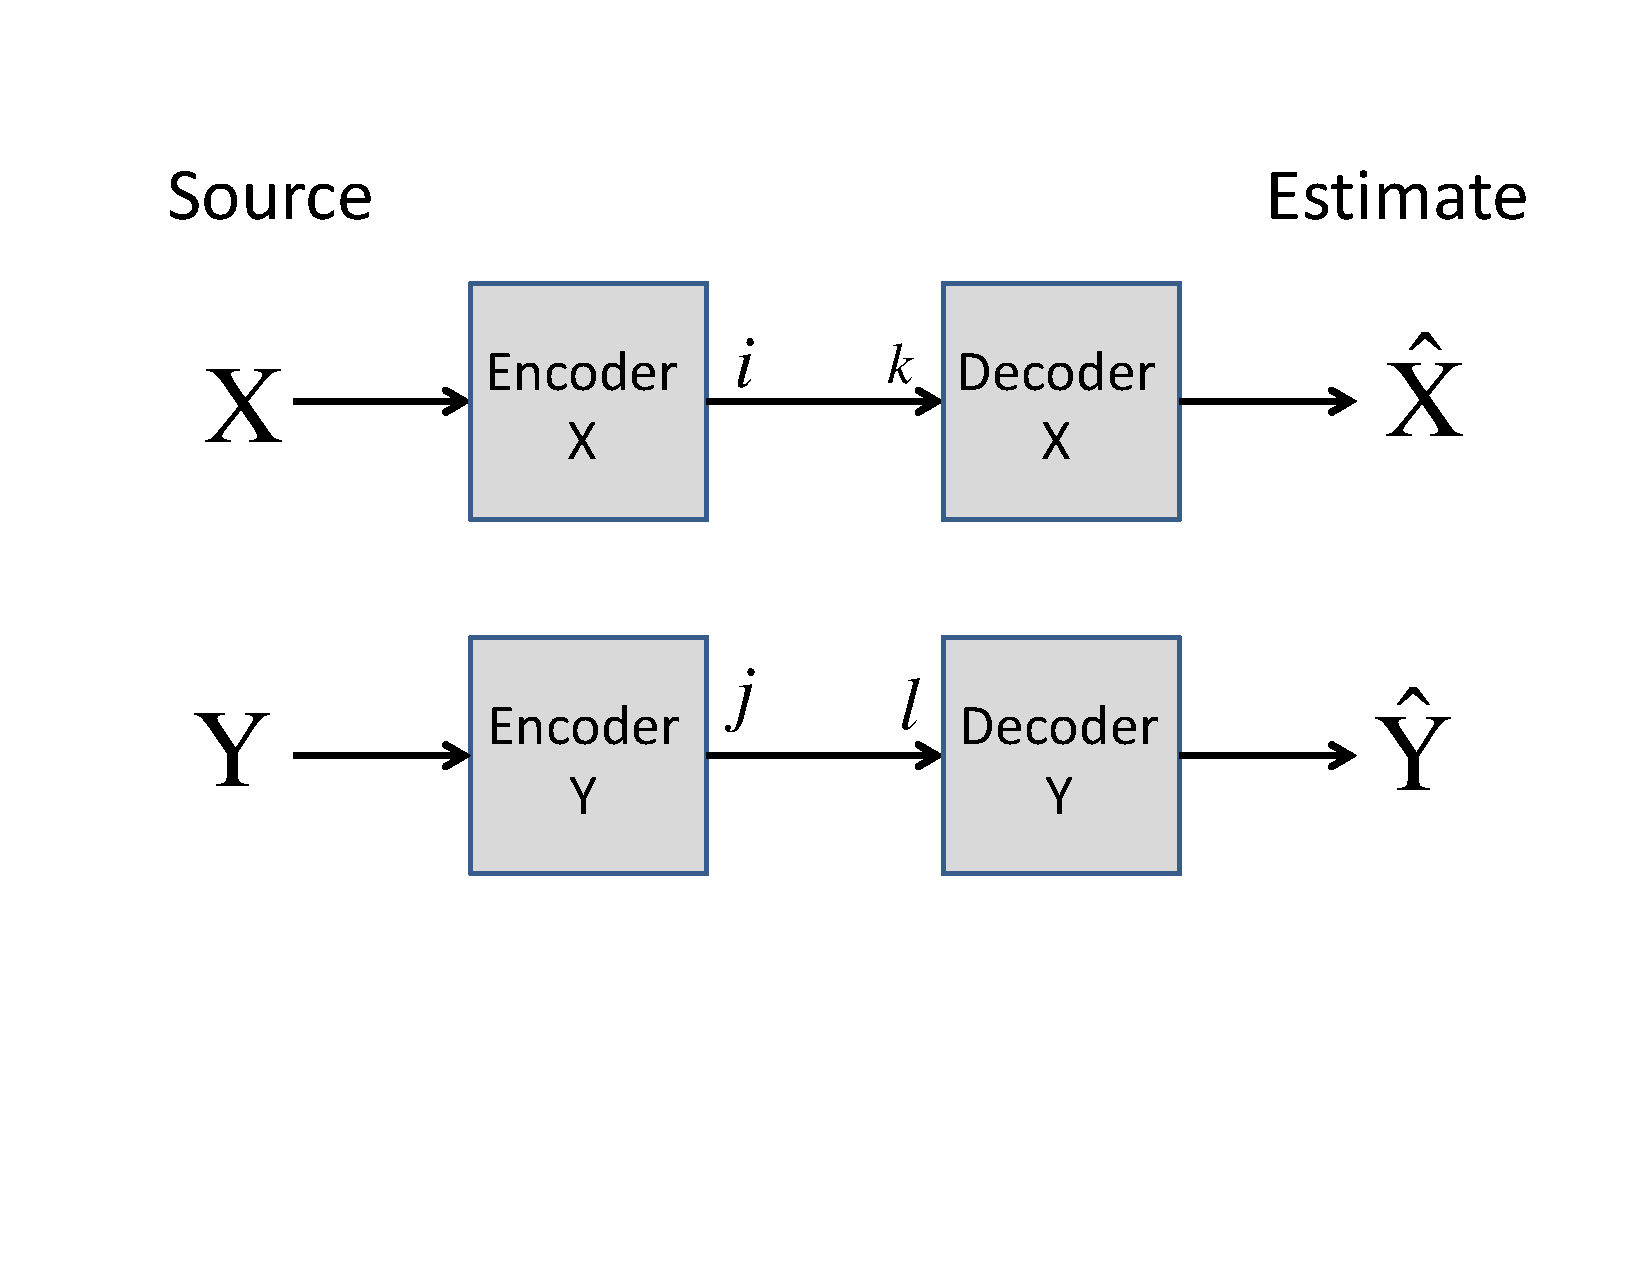
\includegraphics[width=0.4\linewidth]{II.pdf}
    \caption{An illustration of the \sysII\ and \sysIIN\ systems.}
    \label{fig:II_sys}
\end{figure}

\begin{figure}
        \centering
        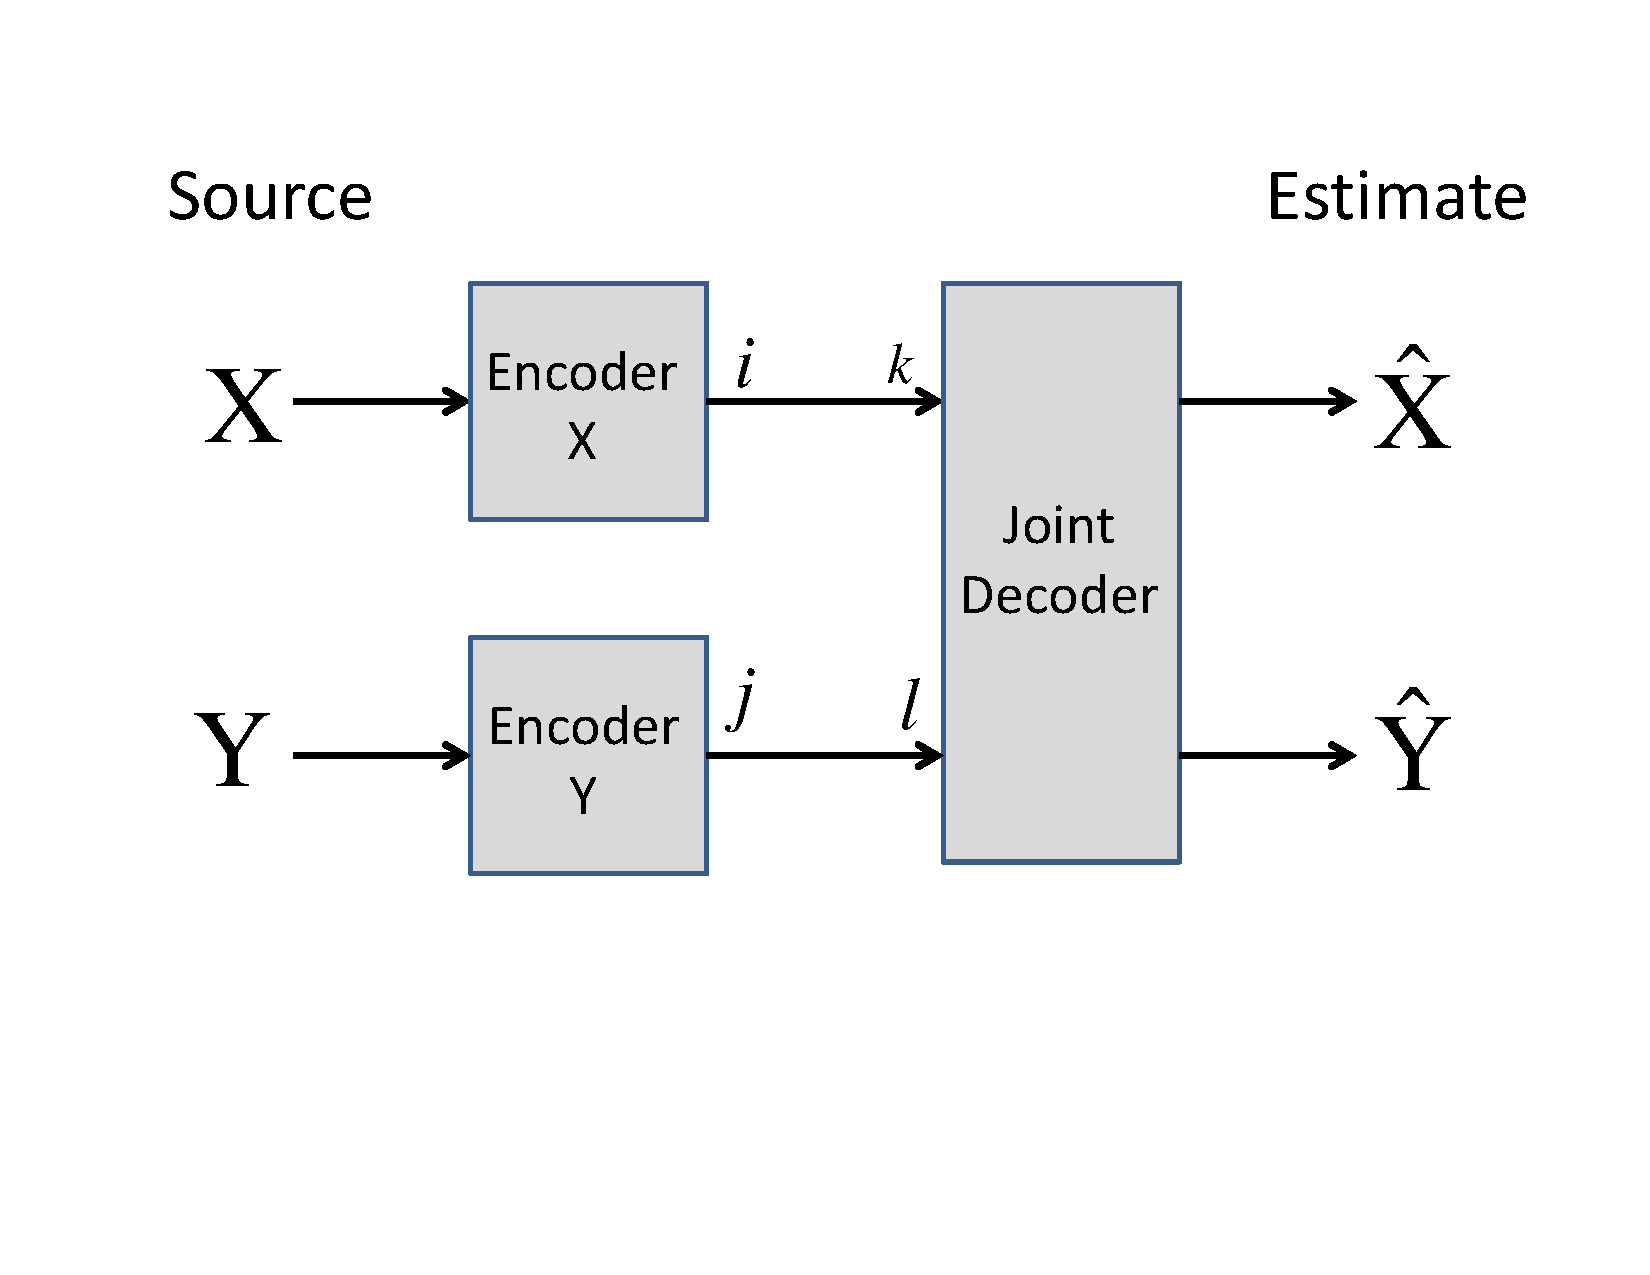
\includegraphics[width=0.4\linewidth]{IJ.pdf}
    \caption{An illustration of the \sysIJ\ and \sysIJN\ systems.}
    \label{fig:IJ_sys}
\end{figure}

\begin{figure}
        \centering
        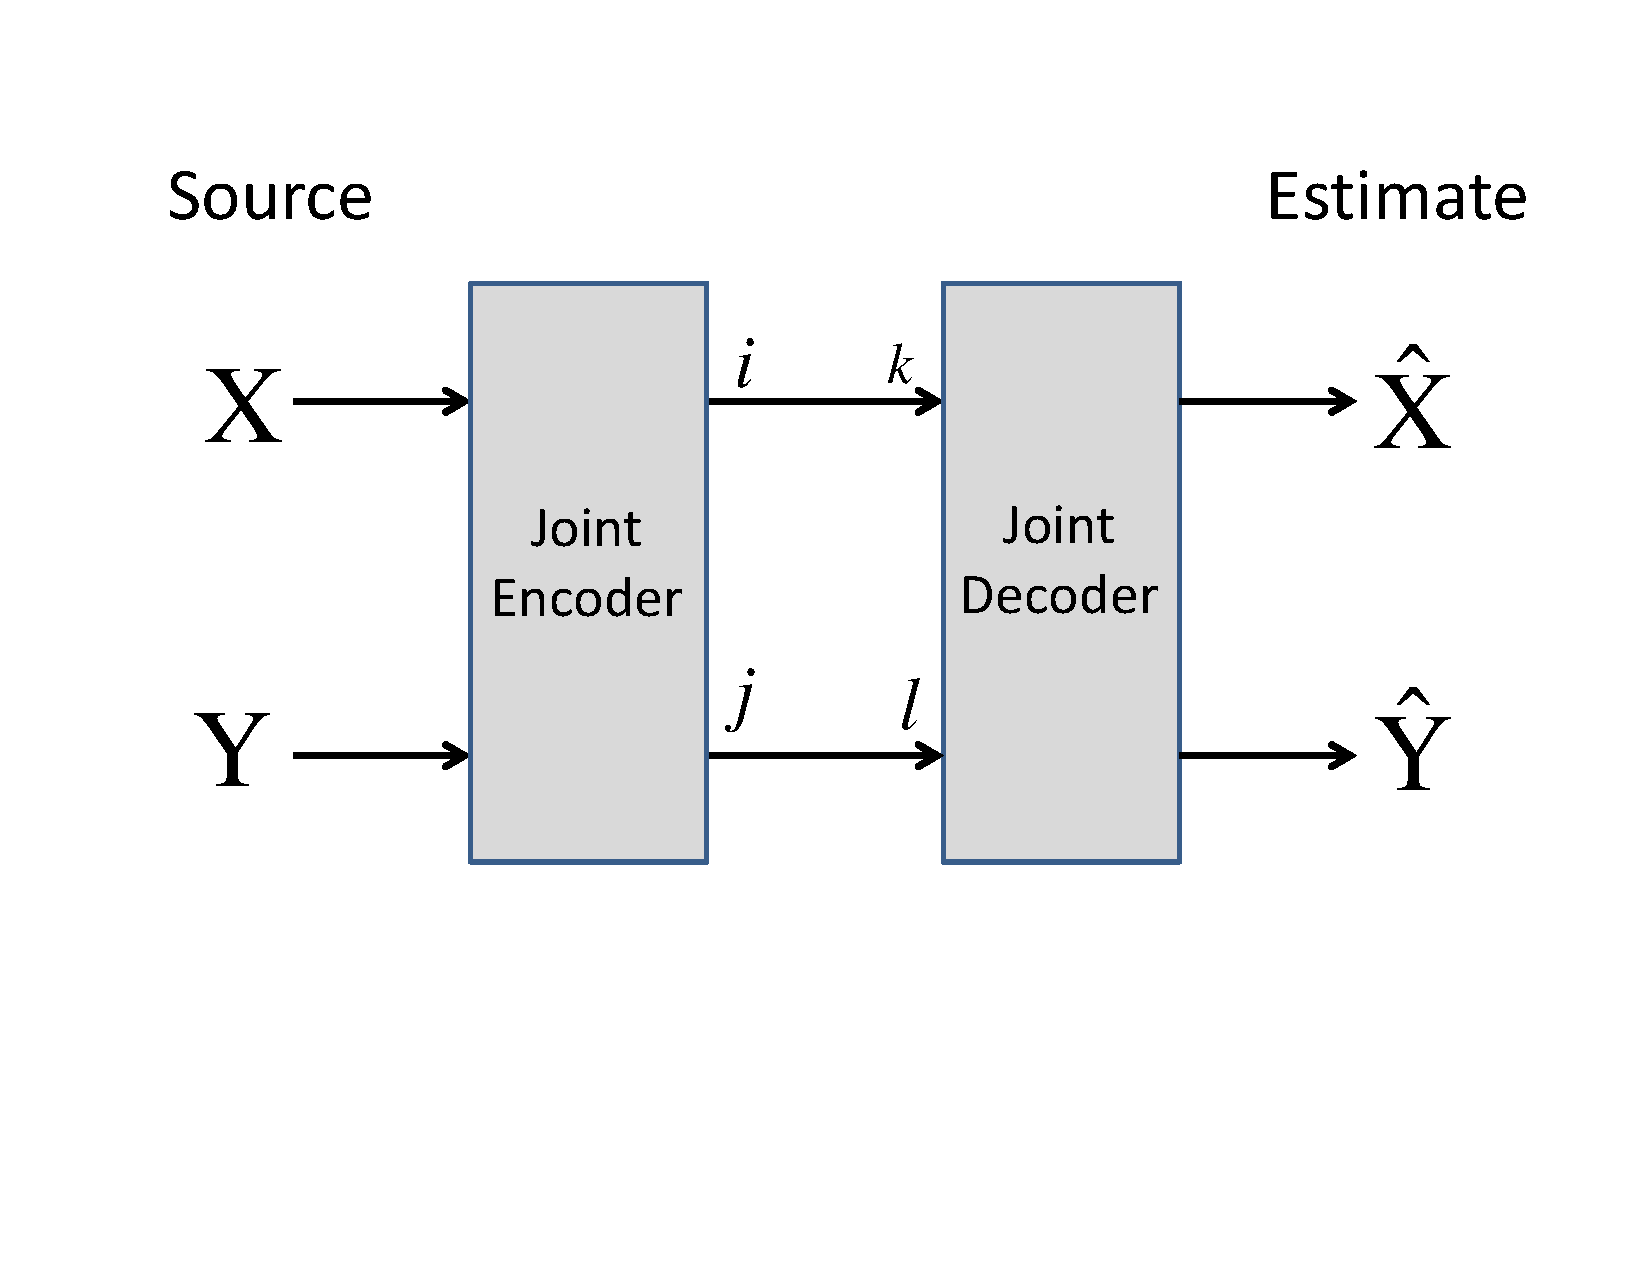
\includegraphics[width=0.4\linewidth]{JJ.pdf}
    \caption{An illustration of the \sysJJ\ and \sysJJN\ systems.}
    \label{fig:JJ_sys}
\end{figure}

The goal of this study is to design and implement \sysIJ\ and \sysIJN\ quantizers and compare their performance against the other quantizer in this two-transmitter system. Schematics for these systems are provided in Figures~\ref{fig:II_sys}, Figures~\ref{fig:IJ_sys}, and Figures~\ref{fig:JJ_sys}.

\subsection{Explicit Expressions for Average Distortion}
The average distortion in (\ref{eq:sys_dist}) will now be re expressed using explicit expressions for the six systems. All of these expressions can be easily derived by conditioning on transmitted and received indices. 

\medskip
{\sc \noindent Independent Encoders And Decoders, No Noise (\sysII):}
\begin{equation}
    \label{eq:dist_indep_nonoise}
    D_{avg} = \sum_{i=1}^{N_X}E[{(X-x_i)}^2 | x \in R_i]P(x \in R_i) + \sum_{j=1}^{N_Y}E[{(Y-y_j)}^2 | y \in S_j]P(y \in S_j)
\end{equation}
The average distortion can be expressed as the sum of distortions between both sources. Moreover, each term on the right-hand side can be minimized independently using two independent scalar quantizers: one for $X$ and one for $Y$.

\medskip
{\sc \noindent Independent Encoders And Decoders, With Noise (\sysIIN):}
\begin{equation}
    \label{eq:dist_indep_noise}
    D_{avg} = \sum_{i=1}^{N_X}\sum_{j=1}^{N_Y}\sum_{k=1}^{N_X}\sum_{l=1}^{N_Y}
    E[{(X-x_{k})}^2 + {(Y-y_{l})}^2 | X \in R_i, Y \in S_j]P(b_X(k),b_Y(l)|b_X(i),b(j))P(X \in R_i, Y \in R_j)
\end{equation}
Here the notation $b_X$ and $b_Y$ is used to denote the codeword assignment mappings for $X$ and $Y$ respectively. Unlike the previous system, the average distortion for the \sysIIN\ system can not be separated into two separate terms unless it is assumed that the two channels are independent, or $P(b(k),b(l)|b(i),b(j)) = P(b(k)|b(i))P(b(l)|b(j))$. Under this assumption we have
\begin{multline}
    \label{eq:dist_indep_chan}
    D_{avg} = 
    \sum_{i=1}^{N_X}\sum_{k=1}^{N_X} E[{(X-x_{k})}^2 | X \in R_i]P(b_X(k)|b_X(i))P(X \in R_i) + \\
    \sum_{j=1}^{N_Y}\sum_{l=1}^{N_Y} E[{(Y-y_{l})}^2 | Y \in S_j]P(b_Y(l)|b_Y(j))P(Y \in S_j) 
\end{multline}
Two independent channel optimized scalar quantizers can be independently designed to quantize $X$ and $Y$ in order to minimize~(\ref{eq:dist_indep_chan}). Although the assumption that the two channels are independent is not necessary in order to study the nature of the other channels, only independent channels will be studied in this paper so performance can be compared more easily between the different systems.

\medskip
{\sc \noindent Joint Decoder And Joint Encoder, No Noise (\sysJJ):}
\begin{equation}
  \label{eq:dist_JJ}
    D_{avg} = \sum_{i=1}^{N_X}\sum_{j=1}^{N_Y} E[{(X-x_{i,j})}^2 + {(Y-y_{i,j})}^2 | (X,Y) \in R_{i,j}]P((X,Y) \in R_{i,j})
\end{equation}
The above expression can be minimized using a 2-dimensional vector quantizer with codebook size $N_XN_Y$. This can be done by enumerating the different combinations of the $i$s and $j$s.

\medskip
{\sc \noindent Joint Decoder And Joint Encoder, With Noise (\sysJJN):}
\begin{equation}
    D_{avg} = \sum_{i=1}^{N_X}\sum_{j=1}^{N_Y}\sum_{k=1}^{N_X}\sum_{l=1}^{N_Y} E[{(X-x_{k,l})}^2 +
    {(Y-y_{k,l})}^2 | (X,Y) \in R_{i,j}]P(b_X(k),b_Y(l)|b_X(i),b_Y(j))P((X,Y) \in R_{i,j})
\end{equation}
The above expression can be minimized using a 2-dimensional channel optimized quantizer with codebook size $N_XN_Y$. Again, the $i$s and $j$s can be considered to be enumerated.

\medskip
{\sc \noindent Independent Encoders And Joint Decoders, No Noise (\sysIJ):}
\begin{equation}
    \label{eq:dist_IJ}
    D_{avg} = \sum_{i=1}^{N_X}\sum_{j=1}^{N_Y} E[{(X-x_{i,j})}^2 + {(Y-y_{i,j})}^2 | X \in R_i, Y \in S_j]P(X \in R_i, Y \in S_j)
\end{equation}
Notice the slight difference between this expression and that of~(\ref{eq:dist_JJ}). New conditions for optimality will be derived for this system in the next subsection and the implementation of such a quantizer will be discussed in detail in the following section. 

\medskip
{\sc \noindent Independent Encoders And Joint Decoders, With Noise (\sysIJN):}
\begin{equation}
    \label{eq:dist_IJN}
    D_{avg} = \sum_{i=1}^{N_X}\sum_{j=1}^{N_Y}\sum_{k=1}^{N_X}\sum_{l=1}^{N_Y} E[{(X-x_{k,l})}^2 +
    {(Y-y_{k,l})}^2 | X \in R_i, Y \in S_j]P(b_X(k),b_Y(l)|b_X(i),b_Y(j))P(X \in R_i, Y \in S_j)
\end{equation}
This represents the distortion for our other independent encoder/joint encoder system, this time with channel noise. 

Many of the analogies made between the \sysIJ\ system and \sysJJ\ systems made above also apply between the \sysIJ\ and \sysIJN\ systems. In particular, the expression for average distortion for the \sysIJN\ system can not be separated into two independent terms, and the encoders and joint decoder have to be designed together.

The new conditions of optimality used in the \sysIJ\ and \sysIJN\ systems will now be introduced. A detailed description of the design algorithm for these two systems will follow in the next section.

\subsection{Conditions of Optimality}
Conditions of optimality for the \sysIJ\ and \sysIJN\ systems will now be discussed beginning with the centroid condition. Beginning with the \sysIJ\ system, one can see from (\ref{eq:dist_IJ}) that the optimal code vectors are given by
\begin{align}
x_{i,j} &= E[X | X \in R_i, Y \in R_j] \\
&= \frac{ \int_{S_j}\int_{R_i}xf(x,y)dxdy }{ \int_{S_j}\int_{R_i}f(x,y)dxdy } \\
\end{align}
and
\begin{align}
y_{i,j} &= E[Y | Y \in R_i, Y \in R_j] \\
&= \frac{ \int_{S_j}\int_{R_i}yf(x,y)dxdy }{ \int_{S_j}\int_{R_i}f(x,y)dxdy } \\
\end{align}
These equations are analogous to the equations for the centroid condition derived for the quantizer in (\ref{eq:cent_vq}). Similar equations can be given for the centroids for the \sysIJN\ system:
\begin{align}
  x_{k,l} &= \frac{\sum_{i=1}^{N_X} \sum_{j=1}^{N_Y} P(b_X(k),b_Y(l)|b_X(i),b_Y(j))E[X | X \in R_i, Y \in R_j] P(X \in R_i, Y \in R_j)}
{\sum_{i=1}^{N_X} \sum_{j=1}^{N_Y} P(b_X(k),b_Y(l)|b_X(i),b_Y(j))P(X \in R_i, Y \in R_j)}  \nonumber\\
\label{eq:cent_x}
  &= \frac{\sum_{i=1}^{N_X} \sum_{j=1}^{N_Y} P(b_X(k),b_Y(l)|b_X(i),b_Y(j))\int_{S_j} \int_{R_i} xf(x,y)dxdy}
{\sum_{i=1}^{N_X} \sum_{j=1}^{N_Y} P(b_X(k),b_Y(l)|b_X(i),b_Y(j))\int_{S_j} \int_{R_i} f(x,y)dxdy}
\end{align}
and
\begin{align}
  y_{k,l} &= \frac{\sum_{i=1}^{N_X} \sum_{j=1}^{N_Y} P(b_X(k),b_Y(l)|b_X(i),b_Y(j))E[Y | X \in R_i, Y \in R_j] P(X \in R_i, Y \in R_j)}
{\sum_{i=1}^{N_X} \sum_{j=1}^{N_Y} P(b_X(k),b_Y(l)|b_X(i),b_Y(j))P(X \in R_i, Y \in R_j)} \nonumber\\
\label{eq:cent_y}
  &= \frac{\sum_{i=1}^{N_X} \sum_{j=1}^{N_Y} P(b_X(k),b_Y(l)|b_X(i),b_Y(j))\int_{S_j} \int_{R_i} yf(x,y)dxdy}
{\sum_{i=1}^{N_X} \sum_{j=1}^{N_Y} P(b_X(k),b_Y(l)|b_X(i),b_Y(j))\int_{S_j} \int_{R_i} f(x,y)dxdy}
\end{align}
Again, these equations are similar to the centroid condition for the channel optimized vector quantizer in (\ref{eq:cent_covq}).

The nearest neighbor conditions for the \sysIJ\ system will now be given. Let $d_X(x,i)$ denote the expected distortion given $X=x$ and index $i$ was encoded at the $X$ encoder:
\begin{equation}
d_X(x,i)= \sum_{j=1}^{N_Y} ( {(x-x_{i,j})}^2 + E[{(Y-y_{i,j})}^2|X=x,Y\in S_j])P(Y \in S_j|X=x)
\end{equation}
Let $d_Y(y,j)$ denote a similar expression for $Y$:
\begin{equation}
d_Y(y,j)= \sum_{i=1}^{N_X} ( {(y-y_{i,j})}^2 + E[{(X-x_{i,j})}^2|Y=y,X\in R_i])P(X \in R_i|Y=y)
\end{equation}

The nearest neighbor condition for the \sysIJ\ system is given as follows:

\begin{theorem}
  \label{theo:NN_IJ}
Amongst all \sysIJ\ systems with codebooks $\mathcal{C}_X$, $\mathcal{C}_Y$and $Y$ encoder $\mathcal{E}_Y$, the system whose $X$ encoder $\mathcal{E}_X$ has encoding regions satisfy
\begin{equation}
R_i \subset \{ x : d_X(x,i) \le d_X(x,j) \text{ for all } j=1,\ldots,N_X \}
\end{equation}
for all $i=1,\ldots,N_X$ is optimal.
\end{theorem}

A similar theorem also applies to the $Y$ encoder $\mathcal{E}_Y$, using $d_Y(y,j)$ instead of $d_X(x,i)$.

\medskip

For the \sysIJN\ system, let  $d_X^N(x,i)$ denote the expected distortion at the receiver given $X=x$ and index $i$ was transmitted:
\begin{equation}
d_X^N(x,i)= \sum_{j=1}^{N_Y} \sum_{k=1}^{N_X} \sum_{l=1}^{N_Y} ( {(x-x_{k,l})}^2 + E[{(Y-y_{k,l})}^2|X=x,Y\in S_j])P(Y \in S_j|X=x) P(b_X(k),b_Y(l)|b_X(i),b_Y(j))
\end{equation}
Similarly, let $d_Y^N(y,j)$ denote the expected distortion at the receiver given $Y=y$ and index $j$ was transmitted:
\begin{equation}
d_Y^N(y,j)= \sum_{i=1}^{N_X} \sum_{k=1}^{N_X} \sum_{l=1}^{N_Y} ( {(y-y_{k,l})}^2 + E[{(X-x_{k,l})}^2|Y=y,X\in R_i])P(X \in R_i|Y=y) P(b_X(k),b_Y(l)|b_X(i),b_Y(j))
\end{equation}

Theorem~\ref{theo:NN_IJ} can be adapted to the \sysIJN\ system by using $d_X^N(x,i)$ and $d_Y^N(y,j)$ instead of $d_X(x,i)$ and $d_Y(y,j)$.

It is important to note that Theorem~\ref{theo:NN_IJ} differs from the nearest neighbor conditions for vector quantization and channel optimized quantization. This is because for the \sysIJ\ and \sysIJN\ systems the two encoders, $\mathcal{E}_X$ and $\mathcal{E}_Y$, depend on the other encoder being fixed, and also dependent on the source distribution, rather than just the codebook as before. This has implications in terms of application as well. The Lloyd-Max algorithm has to be adjusted to account for this by alternating between three steps: the centroid condition and the two nearest neighbor conditions for each source. These issues, and how they are dealt with, are discussed  in the following section.

\section{System Design and Implementation}
\label{sec:design}
The new conditions of optimality presented above for the \sysIJ\ and \sysIJN\ systems introduce some new design challenges. In the subsequent sections we will detail the design problems that were faced along the way towards implementation, and how they were addressed.

During this project, we began by writing a C program implement the \sysII\ system, and then adapted it for the \sysIIN\ system by modifying the conditions of optimality as  outlined in the previous section. We then wrote a C program of the \sysIJ\ system without channel noise. To interface with images, we wrote a Python wrapper program. GNU Octave, MathWorks MATLAB, and Python were used to produce data and create plots.

\subsection{Conditions of Optimality}
We begin by writing out the nearest neighbor conditions for the \sysIJN\ system. To begin, the expressions for $d_X^N(x,i)$ and $d_Y^N(y,j)$ are expanded as follows:
\begin{align}
    \label{eq:int_dist_x}
    d_X^N(x,i)=&E[Y^2 | X = x] +\\
    &\sum_{j=1}^{N_Y} \sum_{k=1}^{N_X} \sum_{l=1}^{N_Y} ( {(x-x_{k,l})}^2 -
    2y_{k,l}E[Y|X=x,Y\in R_j^Y] + y_{k,l}^2 )P(Y\in R_j^Y|X=x)
    P(k,l|i,j)\nonumber\\
    \label{eq:int_dist_y}
        d_Y^N(y,j)=&E[X^2 | Y = y] +\\
    &\sum_{i=1}^{N_X} \sum_{k=1}^{N_X} \sum_{l=1}^{N_Y} ( {(y-y_{k,l})}^2 -
    2x_{k,l}E[X|Y=y,X\in R_i^X] + x_{k,l}^2 )P(X\in R_i^X|Y=y)
    P(k,l|i,j)\nonumber
\end{align}

It is important to note how the nearest neighbor condition for $X$ depends on the $Y$ encoding, and vice versa. It was therefore necessary to adapt the Lloyd-Max iteration because this means the two nearest neighbor conditions cannot be applied at the same time. Instead, it must be applied in three stages: (1) application of the nearest neighbor condition to $X$, (2) application of the nearest neighbor condition to $Y$, and (3) application of the centroid condition for the codebook.

Evaluation  of the expectations and probabilities in \eqref{eq:int_dist_x} and \eqref{eq:int_dist_y} present some new design challenges when dealing with a training set. The problematic terms are
\begin{align}
    \label{eq:problem_1}
    E[Y^2 | X = x]\\
    \label{eq:problem_2}
    E[Y|X=x,Y\in R_j^Y]\\
    \label{eq:problem_3}
    P(Y\in R_j^Y|X=x)
\end{align}

Each of these terms will need to be approximated using the training set for a given value of $x$. In particular, they each require an approximation of the conditional density function $f_{Y|X}(y|X=x)$. Our approach is to first approximate the joint density by a probability mass function (pmf) for $X$ and $Y$, from which the conditional density can be computed. This pmf is obtained by binning the two dimensional training set using a uniform quantizer. Details of this scheme are given in an Appendix.
 
For simplicity of design, the $X$ and $Y$ sources are initially fed through this uniform quantizer before performing the \sysIJN\ , (\sysIJ) training, or simulation. It is important to note that this design simplification affects the values of the distortions of  \eqref{eq:int_dist_x} and \eqref{eq:int_dist_y} as well as the centroids which are discussed later in this section. In particular, conditions of optimality are now applied to the uniformly quantized sources. This leads to the following approximations of the nearest neighbor functions using the uniformly quantized training set: 
\begin{align}
    \label{eq:NN_X}
    d_{\bar X}(\bar x_m,i) &=
            T_{\bar X}(\bar x_m) + 
            \sum_{j=1}^{N_Y} \sum_{k=1}^{N_X} \sum_{l=1}^{N_Y}
            \left(\left({(\bar x_m-x_{k,l})}^2 +
            y_{k,l}^2\right)M_{\bar X}(\bar x_m,j) -2y_{k,l}S_{\bar X}(\bar x_m,j)\right)P(k,l|i,j)
    \\
    \label{eq:NN_Y}
    d_{\bar Y}(\bar y_n,j) &=
            T_{\bar Y}(\bar y_n) + 
            \sum_{i=1}^{N_X} \sum_{k=1}^{N_X} \sum_{l=1}^{N_Y}
            \left(\left({(\bar y_n-y_{k,l})}^2 +
            x_{k,l}^2\right)M_{\bar Y}(\bar y_n,i) -2x_{k,l}S_{\bar Y}(\bar y_n,j)\right)P(k,l|i,j)
\end{align}
where $i=1,\ldots,N_X$, $j=1,\ldots,N_Y$ and $\bar x_m\in \{\bar x_1,\ldots,\bar x_{L_X}\}$, $\bar y_n\in \{\bar y_1,\ldots,\bar y_{L_Y}\}$ represent values from the uniformly quantized input space. The terms $T_{\bar X}(\bar x_m)$, $M_{\bar X}(\bar x_m,j)$, and $S_{\bar X}(\bar x_m,j)$ are the numerical approximations to \eqref{eq:problem_1}, \eqref{eq:problem_2}, and \eqref{eq:problem_3} respectively. They are explicitly defined using the quantized training set as described in an Appendix. Similar explanations apply to the corresponding terms in \eqref{eq:NN_Y}.

Equations \eqref{eq:NN_X} and \eqref{eq:NN_Y} are now computable for given pair $(\bar x_m, i)$ or $(\bar y_n, j)$. The encoders $\mathcal{E}_X$ and $\mathcal{E}_Y$ can now be constructed by applying the nearest neighbor condition, which now reduces to a search over the transmission indices to minimize $d_{\bar X}(\bar x_m,i)$ and $d_{\bar Y}(\bar y_n,j)$ for fixed values of $\bar x_m$ and $\bar y_n$. Note that the terms $M_{\bar X}(\bar x_m,j)$, $S_{\bar X}(\bar x_m,j)$, $T_{\bar X}(\bar x_m)$, and their  $\bar Y$ counterparts (i.e., $M_{\bar Y}(\bar y_n,i)$, $S_{\bar Y}(\bar y_n,i)$ and $T_{\bar Y}(\bar y_n)$) can be computed initially to reduce the computational complexity of the nearest neighbour search.

As mentioned above, applying the uniform quantizer at the beginning of our system also modifies the calculation of the centroids. Recalling equations~\eqref{eq:cent_x} and \eqref{eq:cent_y}, the centroid equations, in terms of the uniformly quantized training set, are as follows:
\begin{align}
    \label{eq:C_X}
    x_{k,l} = 
        \frac{\sum_{i=1}^{N_X} \sum_{j=1}^{N_Y}
        S_{(i,j)}^{\bar X} P(k,l|i,j)}
        {\sum_{i=1}^{N_X} \sum_{j=1}^{N_Y}
        M_{(i,j)} P(k,l|i,j)}\\
    \label{eq:C_Y}
    y_{k,l} = 
        \frac{\sum_{i=1}^{N_X} \sum_{j=1}^{N_Y}
        S_{(i,j)}^{\bar Y} P(k,l|i,j)}
        {\sum_{i=1}^{N_X} \sum_{j=1}^{N_Y}
        M_{(i,j)} P(k,l|i,j)}
\end{align}
The terms $M_{(i,j)}$, $S_{(i,j)}^{\bar X}$ and $S_{(i,j)}^{\bar Y}$ correspond to approximations of the terms $P(X \in R_i, Y \in R_j)$, $E[X|X \in R_i^X, Y \in R_j^Y]$, and $E[Y|X \in R_i^X, Y \in R_j^Y]$ respectively. See Appendix for a detailed description of these terms.

Adding the uniform quantizer to the system (a sort of `pre-quantizer') presents us with new parameters which define the granularity of quantization and its range. These are  the choice of $\bar x_1$, $\bar y_1$, $\bar x_{L_X}$, $\bar y_{L_Y}$, $L_X$ and $L_Y$ from the definitions of $q_X$ and $q_Y$. For our simulations, we chose to (i) center the quantizer about the sample mean of $\mathcal T$, (ii) pick $\{\bar x_1, \bar y_1, \bar x_{L_X}, \bar y_{L_Y}\}$ such that all the training points lie within the range of the quantizer. With these decisions, the only remaining parameter is the number of bins, which controls the granularity of the uniform quantizer.

For a given training set $\mathcal T$, we want fine enough quantization so as  not to distort  \eqref{eq:NN_X} and \eqref{eq:NN_Y} from the true source-to-reconstruction distortions, but coarse enough so that the conditional probabilities are estimated reliably. It is clear that with a larger training set $\mathcal T$, we can use finer quantizations while maintaining reliably estimated bins. For our purposes, we iterate through values of $L_X, L_Y$, choosing the result resulting in lowest average distortion.

It is also important to note that the computational complexity depends primarily on  $L_X$ and $L_Y$, not the size of $\mathcal T$, as was the case in the \sysII\ system.

To summarize this section, we present the procedure which we call the `Channel Optimized Stage' of our algorithm. Assuming we are provided an initial codebook $\mathcal{C}$, and encoding mappings $\mathcal E_{\bar X}, \mathcal E_{\bar Y}$, we apply our modified Lloyd-Max algorithm to obtain a better set of encoding mappings and codebook as follows:

\begin{enumerate}
    \item Store the previous distortion value, $D_{avg}$.
    \item Quantize the training set $\mathcal T$ to $\mathcal{\bar T}$
    \item Update the $\mathcal{E}_{\bar X}$ by minimizing $d_{\bar X}(\bar x_m,i)$ across $i$ for each $\bar x_m \in \{\bar x_1,\ldots,\bar x_{L_X}\}$.
    \item Update the $\mathcal{E}_{\bar Y}$ in a similar fashion.
    \item Update the codebook by setting each code vector to the centroid using the equations described above.
    \item Repeat until the average distortion changes less than a desired positive threshold, $\delta$; repeat if
    \begin{align}
        \frac
        {D_{avg} - D^*_{avg}}
        {D_{avg}}
        > \delta
    \end{align}
    where $D_{avg}$ is the distortion of the previous iteration, and the new distortion $D^*_{avg}$ is the new distortion
\end{enumerate}

\subsection{Codebook Initialization}
%Since each nearest neighbor condition depends on the encoding regions of the other source and the codebook $\mathcal C$, and the joint centroid conditions depend on the encoding regions for both sources, it is necessary to find either (a) initial encoding regions $\{R_i^{\bar X}\}, \{S_j^{\bar Y}\}$ for the encoders or (b) initial encoding regions for one of the sources and initial reconstruction points $\{(x_{(k,l)}, y_{(k,l)})\}$ for the decoder. We decided to do both, exploring a of couple strategies.
%
%To make finding initial encoding regions simpler, we took a heuristic approach to firstly initialize a codebook of the desired size, $\mathcal C=\{(x_{(k,l)}, y_{(k,l)})\}$, $k=1\ldots N_X$, $l=1\ldots N_Y$, then apply suitable conditions to find initial encoding regions for \emph{both} sources, and finally begin the main iteration.

Several codebook initialization scheme were tested, but only the best initialization scheme will be discussed in this report. The initialization scheme that was used is an adaption of the Linde-Buzo-Gray (LBG) Splitting Algorithm. Our adaptation is as follows, and is called the 'Initialization Stage'.

The codebook is initialized with a single code vector, $(x_{1,1},y_{1,1})$:
\begin{align}
    x_{1,1} = \sum_{m=1}^{L_X}\sum_{n=1}^{L_Y}\bar x_m p(\bar x_m, \bar y_n)\\
    y_{1,1} = \sum_{m=1}^{L_X}\sum_{n=1}^{L_Y}\bar y_n p(\bar x_m, \bar y_n)
\end{align}
which are the expected values of the uniformly quantized training set $\mathcal T$ for $X$ and $Y$. With only a single possible output, the encoders for each source are given by
\begin{equation}
    \mathcal E_X(x) = \mathcal E_Y(y) = 1
\end{equation}

We then define the average distortion for this choice of codebook as the expected value of the sum of the squared error distortion between the quantized training vectors in $\mathcal T$ and the codebook:
\begin{equation}
    D^*_{avg}=\sum_{m=1}^{L_X}\sum_{n=1}^{L_Y}p(\bar x_m,\bar y_n)\left((\bar x_m-x_{1,1})^2+(\bar y_n-y_{1,1})^2\right)
\end{equation}

We then split in the $X$ and apply a modified Lloyd iteration described as follows.
\begin{enumerate}
    
    \item \label{init_split} Split in $X$: let $N_X=2N_X$
    \item \label{init_start} Remember previous distortion: let $D_{avg}=D^*_{avg}$
    \item Update the $X$ encoder: for each $\bar x_m\in\{\bar x_1,\ldots,\bar x_{L_X}\}$ let
    \begin{align}
        \mathcal E_X(\bar x_m) = \argmin_{i \in \{1,\dots,N_X\}}d_{\bar X}(\bar x_m,i)
    \end{align}
    where $d_{\bar X}(\bar x_m,i)$ is given as in \eqref{eq:NN_X}, however with zero probability of channel error reduces to (this corresponds to the \sysIJ\ system):
    \begin{align}
        \label{eq:no_channel_NN_X}
        d_{\bar X}(\bar x_m,i) =
            T(\bar x_m) + 
            \sum_{j=1}^{N_Y}
            \left(\left({(\bar x_m-x_{i,j})}^2 +
            y_{i,j}^2\right)M(\bar x_m, j) -2y_{i,j}S(\bar x_m, j)\right)
    \end{align}
    \item Repeat the previous step, except for the $Y$ encoder
    \item Update the codebook values: for each $k\in \{1,\ldots,N_X\}$, $l\in\{1,\ldots,N_Y\}$, let
    \begin{align}
        x_{k,l} &= 
            \frac{\sum_{(\bar x_m,\bar y_n)\in R_i^X\times R_j^Y}\bar x_m p(\bar x_m,\bar y_n)}
            {\sum_{(\bar x_m,\bar y_n)\in R_i^X\times R_j^Y}p(\bar x_m,\bar y_n)} \\
        y_{k,l} &= 
            \frac{\sum_{(\bar x_m,\bar y_n)\in R_i^X\times R_j^Y}\bar y_n p(\bar x_m,\bar y_n)}
            {\sum_{(\bar x_m,\bar y_n)\in R_i^X\times R_j^Y}p(\bar x_m,\bar y_n)}
    \end{align}
    Notice that this is the expected value of the partition $(i,j)$.
    \item Compute the new distortion $D^*_{avg}$:
    \begin{enumerate}
        \item
        If
        $\frac
        {(D_{avg} - D^*_{avg})}
        {D_{avg}}
        > \delta$
        then return to step \ref{init_start},
        \item
        otherwise if $N_X$ is less than desired, go to next split (step \ref{init_split}),
        \item
        otherwise finish.
    \end{enumerate}
\end{enumerate}

The above algorithm will give us the desired value of $N_X$; we then apply the symmetric splitting algorithm in $Y$ until we reach our desired codebook size $N_Y$ in the $Y$. This yields an initial codebook optimized with respect to the dependence between $X$ and $Y$. It is worth noting that the properties of the channel do not enter this stage; this was a conscious choice that allows for the channel to not be defined for codebooks of size less than $N_XN_Y$.

When designing the system, we begin with the `Initialization Stage', followed by the `Channel Optimization Stage' which was described in the previous section.
% Implementation:
% Tried Assigning codevectors to first N training points. Didn't work very well
% Tried splitting Algorithm. Advantage: can initialize encoders more easily. Should converge to a more optimal solution.
% Need to consider how to initialize encoders since you can't initialize one encoder using nearest neighbour conditions without having the other one already initialized.
% Splitting makes this simple

\subsection{Codeword Assignment}
% Need to map indices onto binary codewords. Present minimization problem. Problem is NP-complete.
% build this up from point-to-point case
% show minimization objective function of the codeword maps b_X, b_Y
\label{sec:sim_anneal}.
We now discuss codeword assignment for our systems. In particular, these are the mappings $b_X$ and $b_Y$ which map indices onto transmission codewords discussed in Section~\ref{sec:code_assign}. As mentioned in Section~\ref{sec:code_assign}, the technique of simulated annealing is used to estimate good $b_X$ and $b_Y$ mappings. Simulated annealing is a technique used to minimize some energy cost function (this function will be defined shortly for our case). In simulated annealing, one jumps randomly between states (in our case, this corresponds to permutations of the mappings $b_X$ and $b_Y$) while evaluating the energy function. If the energy at a new state is less than before, the change is accepted. If the energy at a new state is higher than before, the new state is only accepted with a certain probability that is a function of a `temperature' variable. This variable is initially set to a high value, so that most changes are accepted. The temperature is gradually reduced over time, which corresponds to less states being accepted. The idea of simulated annealing is to avoid local optima by gradually decreasing temperature. The energy function to be minimized is similar to the one discussed in Section~\ref{sec:code_assign} and is given as follows:
\begin{equation}
    \label{eq:energy}
    D_C(b_X,b_Y)=
        \sum_{i,j}
            \sum_{k,l}
            P(b_X(k), b_Y(l) | b_X(i), b_Y(j))
            \left((x_{i,j}-x_{k,l})^2+(y_{i,j}-y_{k,l})^2\right)
\end{equation}
A detailed implementation of the algorithm is provided in an Appendix, along with parameter values that were used in the process.

\subsection{Image Coding}
% Presented problems with what to input to quantizer -> DCT blocks
% Bit allocation (we did not explore this for joint decoder case)

Given our system was designed for two correlated sources, we decided to apply it to the compression of two images that share spatial correlation. We focus on stereoscopic images in our project, i.e. pairs of images of the same object taken from different angles. We explore the effect of transform coding on pairs of images from this class as input to our system.

Transform coding is often used in practice for efficient image coding. The concept behind transform coding is to perform an \emph{orthogonal} linear transform on large blocks of the source scalars prior to scalar quantization, then inverse transform on the decoding side. The reason this is done is to pairwise \emph{de-correlate} the components of the input vector such that the components of the output vector of the transform are (close to) pairwise uncorrelated.

Of the known computable orthogonal linear transforms, the Discrete Cosine Transform (DCT) has been found to be the most effective, and it is widely used in image and video compression. A 2-D DCT is often used on blocks of 8$\times$8 pixels of the source image before scalar quantization of each component. This is similar to the scheme used in JPEG compression. The 64 coefficients are then provided as input to our quantizer either as a training set to train the encoding regions and codebook, or as a simulation set to be encoded by a trained encoder. Recall that each DCT coefficient comes in a pair, where there is one coefficient per source.

\medskip

\begin{figure}
    \centering
    \begin{subfigure}{0.5\textwidth}
        \centering
        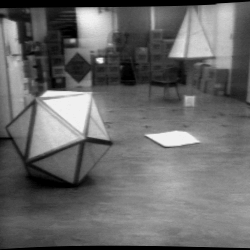
\includegraphics[width=0.6\linewidth]{cart_orig_left.png}
        \caption{left}
    \end{subfigure}% <- this percent sign is important 8)
    \begin{subfigure}{0.5\textwidth}
        \centering
        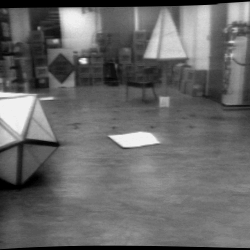
\includegraphics[width=0.6\linewidth]{cart_orig_right.png}
        \caption{right}
    \end{subfigure}
    \caption{An example of a stereo image.}
    \label{fig:cart_orig}
\end{figure}

An example of the type of image we used is shown in Figure~\ref{fig:cart_orig}.

\begin{figure}
    \begin{subfigure}{0.5\textwidth}
        \begin{equation*}
            \left[
            \begin{matrix}
                7 & 7 & 5 & 4 & 0 & 0 & 0 & 0 \\
                7 & 5 & 4 & 0 & 0 & 0 & 0 & 0 \\
                6 & 5 & 0 & 0 & 0 & 0 & 0 & 0 \\
                5 & 0 & 0 & 0 & 0 & 0 & 0 & 0 \\
                5 & 0 & 0 & 0 & 0 & 0 & 0 & 0 \\
                4 & 0 & 0 & 0 & 0 & 0 & 0 & 0 \\
                0 & 0 & 0 & 0 & 0 & 0 & 0 & 0 \\
                0 & 0 & 0 & 0 & 0 & 0 & 0 & 0
            \end{matrix}
            \right]
        \end{equation*}
    \caption{left}
    \end{subfigure}%
    \begin{subfigure}{0.5\textwidth}
        \begin{equation*}
            \left[
            \begin{matrix}
                7 & 6 & 5 & 3 & 0 & 0 & 0 & 0 \\
                7 & 4 & 4 & 0 & 0 & 0 & 0 & 0 \\
                6 & 4 & 0 & 0 & 0 & 0 & 0 & 0 \\
                5 & 0 & 0 & 0 & 0 & 0 & 0 & 0 \\
                5 & 0 & 0 & 0 & 0 & 0 & 0 & 0 \\
                4 & 0 & 0 & 0 & 0 & 0 & 0 & 0 \\
                4 & 0 & 0 & 0 & 0 & 0 & 0 & 0 \\
                0 & 0 & 0 & 0 & 0 & 0 & 0 & 0
            \end{matrix}
            \right]
        \end{equation*}
    \caption{right}
    \end{subfigure}
    \caption{Greedy 64 bit allocation for the DCT coefficients for the two stereo images of Figure~\ref{fig:cart_orig}. }
    \label{fig:cart_bit_alloc}
\end{figure}

An important question in transform coding is that of bit allocation. We wish to know how many bits, i.e. how many code vectors, to assign to each DCT coefficient to optimally recover the source. The case involving a single transmitter and receiver was studied in \cite{julien}. A simple greedy algorithm optimally allocates bits to the DCT coefficients. The algorithm assumes that the $(0,0)$ coefficient (the DC coefficient) is Gaussian, while the other 63 coefficients are Laplacian \cite{julien}. An example of how this algorithm allocates bits to the images of Figure \ref{fig:cart_orig} is given in Figure~\ref{fig:cart_bit_alloc}.

\begin{figure}
    \begin{equation*}
        \left[
        \begin{matrix}
        0.443 & -0.01  & -0.093 & -0.011 & -0.061 &   0.003 & -0.017 &  0.062 \\
        0.416 &  0.006 & -0.011 &  0.014 & -0.031 &  -0.039 &  0.003 & -0.045 \\
        0.498 & -0.061 & -0.01  &  0.074 & -0.034 &  -0.017 &  0.008 &  0.054 \\
        0.438 &  0.027 & -0.008 &  0.074 & -0.016 &   0.022 &  0.006 & -0.004 \\
        0.449 &  0.075 & -0.019 &  0.017 &  0.014 &   0.063 & -0.029 &  0.007 \\
        0.632 &  0.028 & -0.034 & -0.018 &  0.033 &  -0.037 &  0.032 &  0.061 \\
        0.765 &  0.177 & -0.032 & -0.063 & -0.033 &   0.076 & -0.001 &  0.089 \\
        0.679 &  0.148 &  0.028 &  0.04  &  0.046 &  -0.013 &  0.046 &  0.034
        \end{matrix}
        \right]
    \end{equation*}
    \caption{DCT coefficient correlation matrix of the stereo images in Figure \ref{fig:cart_orig}.}
\end{figure}

\begin{figure}
    \begin{equation*}
        \left[
        \begin{matrix}
        0.654 & 0.134 & 0.054 & 0.087 & 0.077 & 0.124 & 0.119 & 0.144 \\
        0.371 & 0.072 & 0.043 & 0.059 & 0.05  & 0.063 & 0.053 & 0.048 \\
        0.273 & 0.067 & 0.065 & 0.06  & 0.055 & 0.05  & 0.062 & 0.059 \\
        0.23  & 0.056 & 0.064 & 0.053 & 0.046 & 0.045 & 0.047 & 0.039 \\
        0.242 & 0.053 & 0.05  & 0.056 & 0.047 & 0.062 & 0.058 & 0.036 \\
        0.213 & 0.064 & 0.064 & 0.05  & 0.061 & 0.052 & 0.045 & 0.059 \\
        0.238 & 0.068 & 0.07  & 0.056 & 0.048 & 0.046 & 0.042 & 0.054 \\
        0.233 & 0.081 & 0.074 & 0.066 & 0.046 & 0.05  & 0.039 & 0.049
        \end{matrix}
        \right]
    \end{equation*}
    \caption{Average DCT coefficient correlation matrix of the dataset of 39 pairs of stereo images.}
\end{figure}

The DCT computations and image manipulation were coded in Python using Pillow Imaging library and numpy. The bit allocation problem for the two source case was not studied. We have thus omitted bit allocation from our simulations, and assigned equal bits to each component when comparing systems.

% Implementation:
% Python PILLOW library & numpy

\subsection{Design Summary}
We summarize below the design of our system for processing images. It should be noted that the data set used for training was not the same set used for simulation. This is to prevent statistical biasing. Also, to obtain the \sysIJ\ system, the quantizer just needs to be designed using the Initialization Stage without the Channel-Optimization Stage, because the channel is noiseless for the \sysIJ\ system.

\medskip
{\noindent \bf Training Phase}
\begin{enumerate}
    \item Choose pairs of stereo images to act as the training sets;
    \item Convert pixel data of stereo images to 64 scalar pair sets of 2-D DCT coefficients;
    \item Uniformly quantize sets;
    \item Perform `Initialization Stage' quantization with splitting on each set;
    \item Perform `Channel-Optimization Stage' quantization until convergence on each set;
    \item Perform simulated annealing to  approximate optimal channel codeword mappings $b_X, b_Y$ on each set;
    \item Return to step 5 until satisfactory distortion is achieved.
\end{enumerate}
\medskip
{\noindent \bf Simulation Phase}
\begin{enumerate}
    \item Choose a pair of stereo images to act as the simulation set;
    \item Convert pixel data of stereo images to 64 scalar pair sets of 2-D DCT coefficients;
    \item Uniformly quantize sets;
    \item Using codebooks and channel codeword maps from training phase, find the nearest neighbor for each quantized level;
    \item Send encoded channel indices over a simulated channel;
    \item Receive indices and decode according to the centroid condition.
\end{enumerate}

\section{Testing and Results}
The results of our simulations are twofold. We firstly ran Gaussian training and simulation sets through our \sysII, \sysIJ, \sysJJ\ systems, using Signal-to-Noise Ratio (SNR) to compare the performances of the three systems, we likewise do the same with our \sysIIN, \sysIJN, \sysJJN\ systems. We then make comparisons between performances of the systems on the class of steroscopic images, and present the resulting Signal-to-Noise ratios and images.
\subsection{Gaussian Data}

\begin{figure}[h]
    \centering
    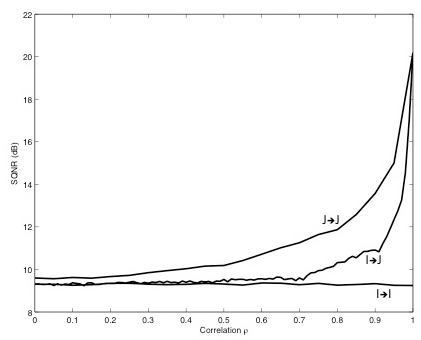
\includegraphics[width=0.65\linewidth]{img/dist_v_rho.png}
    \caption{SQNR as a function of correlation of bivariate Gaussian data for the \sysII\ \sysIJ\ and \sysJJ\ systems.}
    \label{fig:SQNR}
\end{figure}

As was mentioned in the previous section, Gaussian data provide a good model for the constant DCT coefficient of images. It is therefore appropriate to measure the performance of the system on this idealized case before working with actual image sets. We ran three systems: \sysII, \sysIJ, and \sysJJ\ on correlated Gaussian$(0,1)$ training sets, with `outliers', meaning those drawn outside of the square $[-4,4]\times[-4,4]$ removed. The training sets we used were size 250,000. We then simulated the systems on an identically distributed simulation set of size 25,000. We varied the correlation coefficient between 0 and 1 and produced the SQNR-vs-$\rho$ plot of Figure~\ref{fig:SQNR}.

\clearpage
\subsection{Stereoscopic Images}

Below are a few images run through the \sysII, \sysIJ, and \sysJJ\ systems. We begin with the image of Figure~\ref{fig:cart_orig}. When comparing between the systems, we give a constant bit allocation to each of the DCT transform coefficients.

\begin{figure}
    \centering
    \begin{subfigure}{0.5\textwidth}
        \centering
        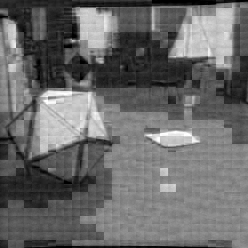
\includegraphics[width=0.6\linewidth]{img/cart_ii_left.png}
        \caption{\sysII\ left: PSNR=11.394 dB}
    \end{subfigure}% <- this percent sign is important 8)
    \begin{subfigure}{0.5\textwidth}
        \centering
        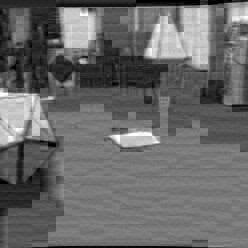
\includegraphics[width=0.6\linewidth]{img/cart_ii_right.png}
        \caption{\sysII\ right: PSNR=12.757 dB}
    \end{subfigure}
    % \caption{\sysII\ trained and simulated on cart.png with constant 2 bit per DCT coefficient allocation}
    \label{fig:cart_ii}

    \centering
    \begin{subfigure}{0.5\textwidth}
        \centering
        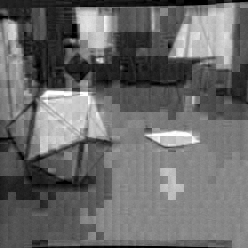
\includegraphics[width=0.6\linewidth]{img/cart_ij_left.png}
        \caption{\sysIJ\ left: PSNR=11.350 dB}
    \end{subfigure}% <- this percent sign is important 8)
    \begin{subfigure}{0.5\textwidth}
        \centering
        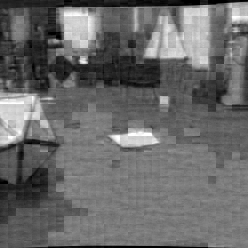
\includegraphics[width=0.6\linewidth]{img/cart_ij_right.png}
        \caption{\sysIJ\ right: PSNR=12.752 dB}
    \end{subfigure}
    % \caption{\sysIJ\ trained and simulated on cart.png with constant 2 bit per DCT coefficient allocation}
    \label{fig:cart_ij}

    \centering
    \begin{subfigure}{0.5\textwidth}
        \centering
        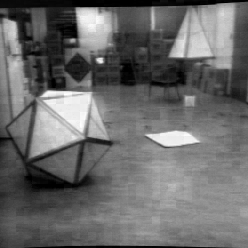
\includegraphics[width=0.6\linewidth]{img/cart_jj_left.png}
        \caption{\sysJJ\ left: PSNR=11.170 dB}
    \end{subfigure}% <- this percent sign is important 8)
    \begin{subfigure}{0.5\textwidth}
        \centering
        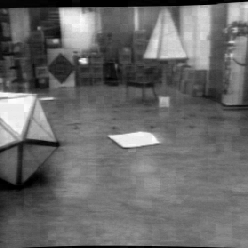
\includegraphics[width=0.6\linewidth]{img/cart_jj_right.png}
        \caption{\sysJJ\ right: PSNR=12.601 dB}
    \end{subfigure}
    \caption{Our three systems trained and simulated on cart.png with constant 2 bit per DCT coefficient allocation}
    \label{fig:cart_jj}
    \label{fig:cart_results}
\end{figure}

\begin{figure}
    \centering
    \begin{subfigure}{0.5\textwidth}
        \centering
        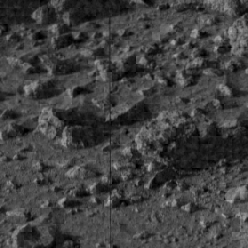
\includegraphics[width=0.6\linewidth]{img/mars1_ii_left.png}
        \caption{\sysII\ left}
    \end{subfigure}% <- this percent sign is important 8)
    \begin{subfigure}{0.5\textwidth}
        \centering
        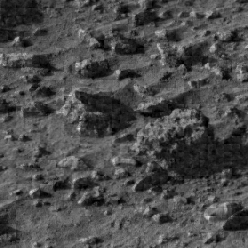
\includegraphics[width=0.6\linewidth]{img/mars1_ii_right.png}
        \caption{\sysII\ right}
    \end{subfigure}
    \caption{Original mars1.png 512$\times$512}
    \label{fig:mars1_orig}
\end{figure}

\begin{figure}
    \centering
    \begin{subfigure}{0.5\textwidth}
        \centering
        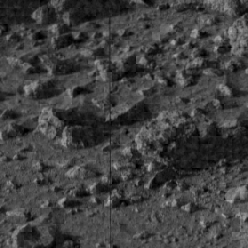
\includegraphics[width=0.6\linewidth]{img/mars1_ii_left.png}
        \caption{\sysII\ left: PSNR=16.738 dB}
    \end{subfigure}% <- this percent sign is important 8)
    \begin{subfigure}{0.5\textwidth}
        \centering
        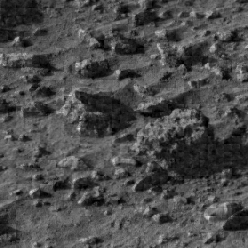
\includegraphics[width=0.6\linewidth]{img/mars1_ii_right.png}
        \caption{\sysII\ right: PSNR=14.825 dB}
    \end{subfigure}
    % \caption{\sysII\ trained and simulated on mars1.png with constant 2 bit per DCT coefficient allocation}
    \label{fig:mars1_ii}

    \centering
    \begin{subfigure}{0.5\textwidth}
        \centering
        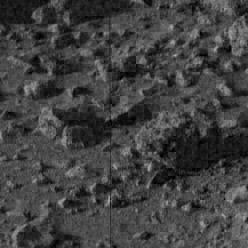
\includegraphics[width=0.6\linewidth]{img/mars1_ij_left.png}
        \caption{\sysIJ\ left: PSNR=16.775 dB}
    \end{subfigure}% <- this percent sign is important 8)
    \begin{subfigure}{0.5\textwidth}
        \centering
        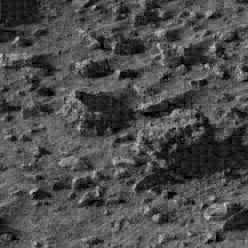
\includegraphics[width=0.6\linewidth]{img/mars1_ij_right.png}
        \caption{\sysIJ\ right: PSNR=14.890 dB}
    \end{subfigure}
    \label{fig:mars1_ij}

    \caption{Our \sysII\ and \sysIJ\ systems trained and simulated on mars1.png}
    \label{fig:mars1_results}
\end{figure}

\begin{figure}
    \centering
    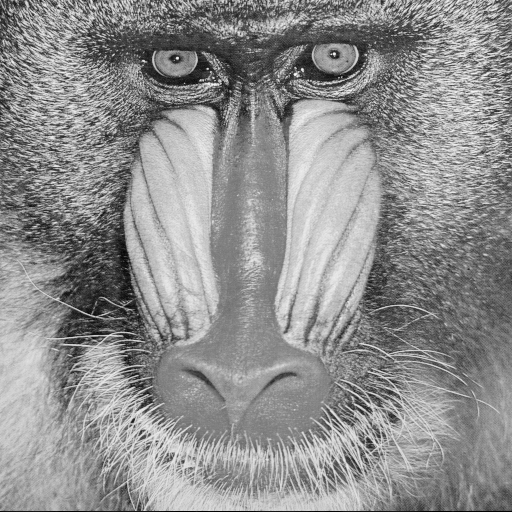
\includegraphics[width=0.6\linewidth]{img/baboon_orig.png}
    \caption{Original baboon.png}
    \label{fig:baboon_orig}
\end{figure}

\begin{figure}
    \centering
    \begin{subfigure}{0.5\textwidth}
        \centering
        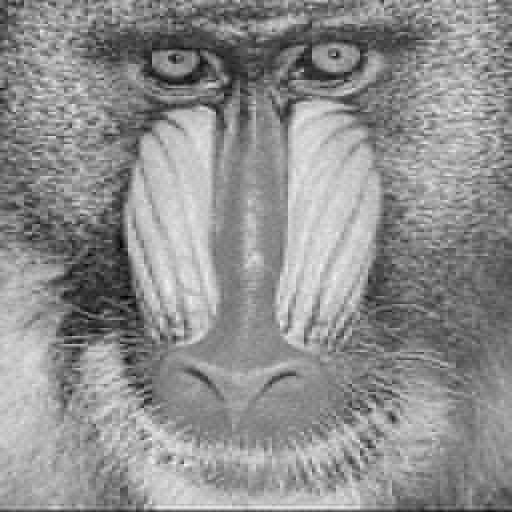
\includegraphics[width=0.6\linewidth]{img/baboon_ii_left.png}
        \caption{\sysII\ left: PSNR=16.833 dB}
    \end{subfigure}% <- this percent sign is important 8)
    \begin{subfigure}{0.5\textwidth}
        \centering
        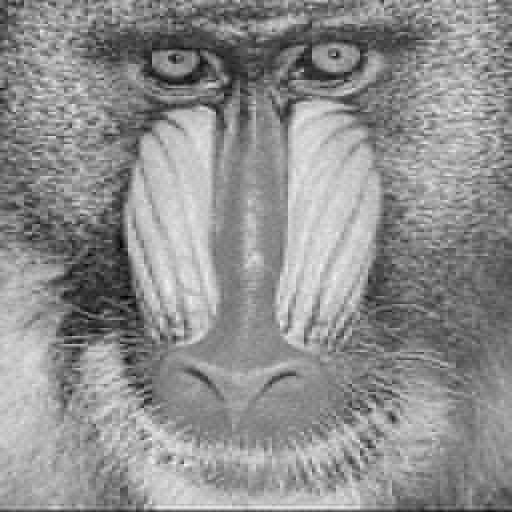
\includegraphics[width=0.6\linewidth]{img/baboon_ii_right.png}
        \caption{\sysII\ right: PSNR=17.446 dB}
    \end{subfigure}
    % \caption{\sysII\ trained and simulated on baboon.png with constant 2 bit per DCT coefficient allocation}
    \label{fig:baboon_ii}

    \centering
    \begin{subfigure}{0.5\textwidth}
        \centering
        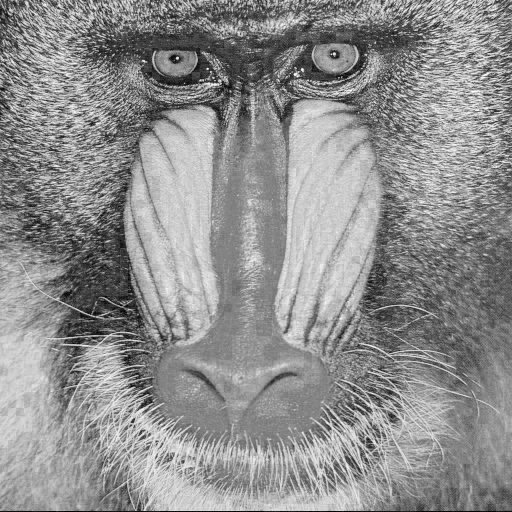
\includegraphics[width=0.6\linewidth]{img/baboon_ij_left.png}
        \caption{\sysIJ\ left: PSNR=20.617 dB}
    \end{subfigure}% <- this percent sign is important 8)
    \begin{subfigure}{0.5\textwidth}
        \centering
        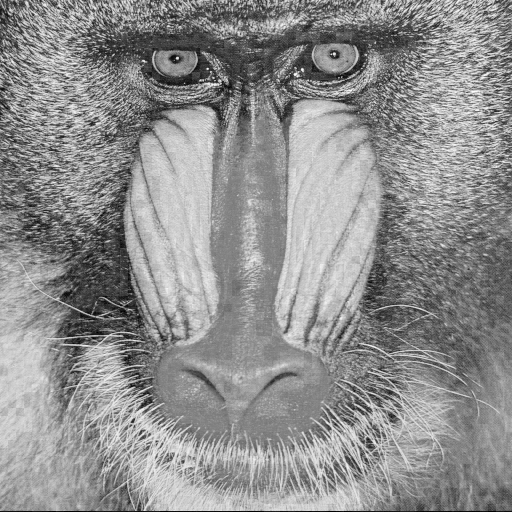
\includegraphics[width=0.6\linewidth]{img/baboon_ij_right.png}
        \caption{\sysIJ\ right: PSNR=20.617 dB}
    \end{subfigure}
    % \caption{\sysIJ\ trained and simulated on baboon.png with constant 2 bit per DCT coefficient allocation}
    \label{fig:baboon_ij}

    \centering
    \begin{subfigure}{0.5\textwidth}
        \centering
        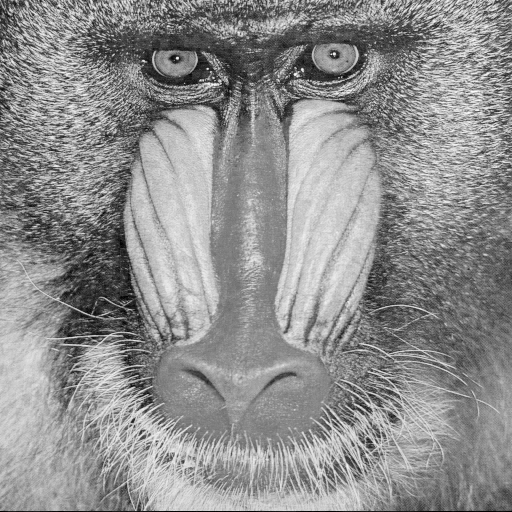
\includegraphics[width=0.6\linewidth]{img/baboon_jj_left.png}
        \caption{\sysJJ\ left: PSNR=34.735 dB}
    \end{subfigure}% <- this percent sign is important 8)
    \begin{subfigure}{0.5\textwidth}
        \centering
        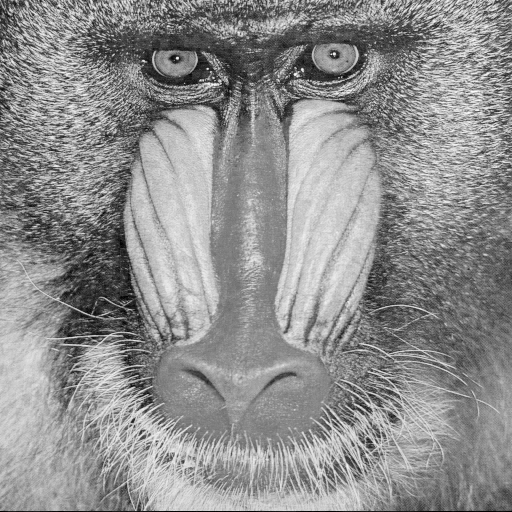
\includegraphics[width=0.6\linewidth]{img/baboon_jj_right.png}
        \caption{\sysJJ\ right: PSNR=34.735 dB}
    \end{subfigure}
    \caption{Our three systems trained and simulated on baboon.png with constant 2 bit per DCT coefficient allocation}
    \label{fig:baboon_results}
\end{figure}

We used 2 bits for each DCT coefficient of each image in every system.  The results of the three systems are given in Figure~\ref{fig:cart_results}.

We ran systems \sysII\ and \sysIJ\ on stereoscopic images taken from Mars.

We also ran the three systems on the ideal case for the \sysIJ\ system: the two sources equal. In Figure \ref{fig:baboon_orig}, we see the standard baboon image in grayscale, and in Figure \ref{fig:baboon_results}, we see the results of our three systems.

\clearpage
\section{Discussion}
The results shown above are now interpreted and evaluated. As mentioned earlier, both generated data and simulated data were used in testing. The most revealing results for the generated data are shown in Figure~\ref{fig:SQNR}. As shown, there were no performance gains for the \sysII\ system as correlation of the bivariate Gaussian data was increased. This is expected because the \sysII\ system does not use source dependence when encoding or decoding.

As expected, the SQNR of the \sysIJ\ system remained above that of the \sysII\ system in Figure~\ref{fig:SQNR}. Notice how the performance of the \sysIJ\ system is approximately the same as that of the \sysII\ system for lower correlations. As correlation increases, benefits of the \sysIJ\ system over the \sysII\ system are only noticeable for $\rho > 0.7$. The performance rapidly increases when this threshold is exceeded.

The \sysJJ\ system outperformed the \sysIJ\ and \sysII\ systems for all values of $\rho$ in Figure~\ref{fig:SQNR}. Again, this is to be expected. One thing to note about the \sysJJ\ system is that benefits from increased correlation are noticed at much lower correlation coefficients than with the \sysIJ\ system. Another thing to note is that when $\rho = 1$, both the \sysIJ\ and \sysJJ\ systems perform equally well. The results illustrated in this graph confirmed our initial assumptions of performance. In particular, it can be seen that the performance of the \sysIJ\ system is bounded by the performance of the \sysII\ and \sysJJ\ systems, and the systems that use a joint decoder benefit from increased source correlation.

Before testing on images, it was noticed that the measured correlation between the DCT coefficient of pairs of stereoscopic images was below the $\rho > 0.7$ needed for performance gains with the generated data. Therefore, it was not expected that the \sysIJ\ system would have much of a performance gain over the \sysII\ system for stereoscopic images. Testing on the stereoscopic images confirmed these expectations. It can be seen in the above images that there is little to no difference in visual performance for the \sysII\ and \sysJJ\ systems.

At this point, it was decided to try using the same image at both sources, thereby having a correlation coefficients of $1$ for all of the DCT coefficient. Large performance gains were expected over the \sysII\ system because of the large SQNR gains that were noticed for the Gaussian data at $\rho=1$. Again, testing confirmed this expectation, and there was a significant visual improvement performance for the \sysIJ\ system over the \sysII\ system in this case.

In conclusion, the benefits of a \sysIJ\ system over a \sysII\ system are only noticeable if the two sources are highly correlated for our design. In practice, it may not be worth implementing a \sysIJ\ system over a \sysII\ system unless the sources are highly correlated. There are also a number of other issues one must consider when implementing a \sysIJ\ system over a \sysII\ system. In particular, the codebook size for the \sysIJ\ system is much larger than the codebook of the \sysII\ system. This may impose memory constraints on the design. Moreover, as seen in the Design section, the nearest neighbor search has a much higher computation complexity for the \sysIJ\ system over the \sysII\ system. 

\section{Summary}
In this study, a network communication system involving two transmitters and a single receiver is investigated. The problem was formulated and a number of different system were considered over both noisy and noiseless channels. Theoretical results for these different systems were investigated to shed light on methods of implementation as well as new conditions of optimality for the independent encoder/joint decoder systems.

The design and implementation of the new systems was built on previous techniques and algorithms in quantizer design. Regardless, the new systems introduces some unique design challenges that had to be overcome and these techniques had to be adjusted accordingly.

In particular, a uniform quantizer was used as a pre-processing step before quantization of the sources in order to estimate the conditional distributions of the sources. Preliminary results indicated that The granularity of this uniform quantizer plays a large role in the overall performance of the system. Therefore, the design was modified by running the entire algorithm over different granularity levels, and picking the one which resulted in lowest distortion. This step drastically improved performance of the system.

Codebook initialization was another design challenge that had to be overcome. The nature of the codebook for the \sysIJ\ and \sysIJN\ systems is a bit different than the other systems because each code vector is represented by two indices. The first initialization scheme that was to initialize the codebook by using the first $N_XN_Y$ points from the training set. It turned out that this did not work very well so the adapted Linde-Buzo-Gray algorithm was used instead.

Encoder initialization was another issue that arose in the design of the \sysIJ\ and \sysIJN\ systems. Recall that for other systems, the encoder can be defined for a fixed codebook by using the nearest neighbor condition. This is not the case for the \sysIJ\ and \sysIJN\ systems because the nearest neighbor condition for one encoder depends on the other encoder. When neither encoder are initialized, it is not possible to apply the nearest neighbor conditions. This problem was overcome by using the adapted Linde-Buzo-Gray algorithm because when the codebook is initialized using a single code vector, the encoders can be initialized by mapping to the single index for that code vector.

All five of the six systems to be studied were successfully implemented. Due to time constraints, however, the \sysIJN\ system was not fully developed. This would be the next step in terms of future work because it is very close to being finished, and it would be interesting to see how noise affects the system. 

Bit allocation was implemented for the \sysII\ and \sysJJ\ systems (that is for vector quantization). Bit allocation for the \sysIJ\ system was not fully investigated, and could offer another route of future study.

More work on the \sysIJ\ system could possibly improve performance at lower correlations. This could make the system more feasible in practical applications, where the sources are not highly correlated. Another avenue of study could be to generalize the two-transmitted one-receiver system to a multiple access channel with an arbitrary number of transmitters. Practical considerations, however, may limit this approach in practice, mainly due to the large codebook size and complexity of the nearest neighbor search.

Finally, better performance may be gained for the stereoscopic images if another transform was applied to the images instead of the DCT. This was not studied closely and could present another avenue of study in the joint-decoder system.

\nocite{*}
\bibliography{thesis_bib}
\section{Appendix:  Evaluation of Optimality Terms}
This appendix details the technical implementation of the uniform quantizer, and the evaluation of some of the conditional values used in the nearest neighbor condition for the \sysIJ\ and \sysIJN\ systems.
Define
$q_X(x):\mathbb{R} \rightarrow \{\bar x_1,\ldots,\bar x_{L_X}\}$
and
$q_Y(y):\mathbb{R} \rightarrow \{\bar y_1,\ldots,\bar y_{L_Y}\}$
to be $L_X$- and $L_Y$-level uniform quantizers for the sources $X$ and $Y$ respectively, where the $\bar x_i-\bar x_{i-1}$ is constant for all $i\in \{2,\ldots,L_X\}$, and $\bar y_i-\bar y_{i-1}$ constant for all $i\in \{2,\ldots,L_Y\}$. Call these constants respectively $\Delta_X, \Delta_Y$.
\begin{align}
    q_X(x) = \bar x_i \in \{\bar x_1,\ldots,\bar x_{L_X}\} &\iff x \in  \left[\bar x_{i}-\frac{\Delta_X}{2},\ \bar x_i+\frac{\Delta_X}{2}\right)\\
    q_Y(y) = \bar y_i \in \{\bar y_1,\ldots,\bar y_{L_Y}\} &\iff y \in  \left[\bar y_{i}-\frac{\Delta_Y}{2},\ \bar y_i+\frac{\Delta_Y}{2}\right)
\end{align}
with the convention that $\bar x_{0}=\bar y_{0}=-\infty$, and $\bar x_{L_X+1}=\bar y_{L_Y+1}=+\infty$.

We begin our approximation by defining the uniformly quantized random variables $\bar X, \bar Y$ as follows:
\begin{align}
    \bar X = q_X(X)\\
    \bar Y = q_Y(Y)
\end{align}

With these uniformly quantized random variables in hand, we can now approximate the conditional densities $f_{Y|X}, f_{X|Y}$ by approximating the conditional pmfs of the $\bar X, \bar Y$ pair with the empirical distributions of a uniformly quantized training set $\mathcal{\bar T}$. Define $\mathcal{\bar T}$ to be the finite training set drawn from the joint pmf of the uniformly quantized pair $\bar X, \bar Y$. Define $p_{\bar Y|\bar X}(\bar y|\bar x),p_{\bar X|\bar Y}(\bar x|\bar y)$ respectively as the conditional \emph{empirical} pmfs of $\bar Y$ given $\bar X$ and $\bar X$ given $\bar Y$ according to the training set $\mathcal{\bar T}$. Our approximation is thus in two stages, namely the uniform quantization step, and the training set estimation step. Each of these contributes in a different way to the approximation error. We have:
\begin{align}
    p_{\bar Y|\bar X}(q_Y(y)|q_X(x)) \approx 
        P(\bar Y=q_Y(y) | \bar X=q_X(x)) \approx
            f_{Y|X}(y|x)\\
    p_{\bar X|\bar Y}(q_X(x)|q_Y(y)) \approx 
        P(\bar X=q_X(x) | \bar Y=q_Y(y)) \approx
            f_{X|Y}(x|y)
\end{align}

Writing out $p_{\bar Y|\bar X}, p_{\bar X|\bar Y}$ in terms of our uniformly quantized training set $\mathcal{\bar T}$ gives:
\begin{align}
    p_{\bar Y|\bar X}(\bar y_n | \bar x_m)=\frac{
            \left|\{(\bar x,\bar y)\in \mathcal{\bar T}\ |\ \bar x = \bar x_m, \bar y = \bar y_n\}\right|
        }{
            \left|\{(\bar x,\bar y)\in \mathcal{\bar T}\ |\ \bar x = \bar x_m\}\right|
        },\quad (\bar x_n, \bar y_m)\in \{x_1,\ldots,x_{L_X}\}\times\{y_1,\ldots,y_{L_Y}\}\\
    p_{\bar X|\bar Y}(\bar x_m | \bar y_n)=\frac{
            \left|\{(\bar x,\bar y)\in \mathcal{\bar T}\ |\ \bar x = \bar x_m, \bar y = \bar y_n\}\right|
        }{
            \left|\{(\bar x,\bar y)\in \mathcal{\bar T}\ |\ \bar y = \bar y_n\}\right|
        },\quad (\bar x_n, \bar y_m)\in \{x_1,\ldots,x_{L_X}\}\times\{y_1,\ldots,y_{L_Y}\}
\end{align}

We now rewrite our approximated versions of equations \eqref{eq:problem_1}, \eqref{eq:problem_2}, \eqref{eq:problem_3} (and their counterparts in $Y$). Define $T_{\bar X}(q_X(x)),T_{\bar Y}(q_Y(y)),M_{\bar X}(q_X(x),j),M_{\bar Y}(q_Y(y),i),S_{\bar X}(q_X(x),j),S_{\bar Y}(q_Y(y),i)$ as these approximations:
\begin{align*}
    T_{\bar X}(q_X(x)) &= \sum_{n=1}^{L_Y}(\bar y_n)^2p_{\bar Y|\bar X}(\bar y_n|q_X(x)) \approx E[Y^2 | X = x]\\
    T_{\bar Y}(q_Y(y)) &= \sum_{m=1}^{L_X}(\bar x_m)^2p_{\bar X|\bar Y}(\bar x_m|q_Y(y)) \approx E[X^2 | Y = y]\\
    M_{\bar X}(q_X(x),j) &= 
        \frac{
            |\mathcal{\bar T}|
        }{
            |\{(\bar x, \bar y)\in \mathcal{\bar T}\ |\ \bar y\in R_j^{\bar Y}\}|
        } \sum_{\bar y_n\in R_j^{\bar Y}}\bar y_np_{\bar Y|\bar X}(\bar y_n|q_X(x))
        \approx E[Y|X=x,Y\in R_j^{Y}]\\
    M_{\bar Y}(q_Y(y),i) &= 
        \frac{
            |\mathcal{\bar T}|
        }{
            |\{(\bar x,\bar y)\in \mathcal{\bar T}\ |\ \bar x\in R_i^{\bar X}\}|
        } \sum_{\bar x_m\in R_i^{\bar X}}\bar xp_{\bar X|\bar Y}(\bar x_m|q_Y(y))
        \approx E[X|Y=y,X\in R_i^{X}]\\
    S_{\bar X}(q_X(x),j) &= 
        \sum_{\bar y_n\in \{\bar y_1,\ldots,\bar y_{L_Y}\}\cap R_j^{\bar Y}}p_{\bar Y|\bar X}(\bar y_n|q_X(x)) 
        \approx P(Y\in R_j^{Y}|X=x)\\
    S_{\bar Y}(q_Y(y),i) &= 
        \sum_{\bar x_m\in \{\bar x_1,\ldots,\bar x_{L_X}\}\cap R_i^{\bar X}}p_{\bar X|\bar Y}(\bar x_m|q_Y(y)) 
        \approx P(X\in R_i^{X}|Y=y)
\end{align*}
Note that we used the notation $R_i^{\bar X}, R_j^{\bar Y}$ to indicate that these are the encoding partitions for the uniformly quantized random variables $\bar X$ and $\bar Y$ respectively.

\section{Appendix B: Evaluation of Centroid Terms}
This appendix details the evaluation of the centroid terms for the \sysIJ\ and \sysIJN\ systems using the quantized training set.
Let $M_{(i,j)}$ be given by:
\begin{align}
    M_{(i,j)} &=
    \sum_{(\bar x_m,\bar y_n)\in R_i^{\bar X}\times R_j^{\bar Y}}p(\bar x_m,\bar y_n)
\end{align}
and let $S_{(i,j)}^{\bar X}$, $S_{(i,j)}^{\bar Y}$ be given by:
\begin{align}
    S^{\bar X}_{(i,j)} &=
    \sum_{(\bar x_m,\bar y_n)\in R_i^{\bar X}\times R_j^{\bar Y}}\bar x_m p(\bar x_m,\bar y_n)\\
    S^{\bar Y}_{(i,j)} &=
    \sum_{(\bar x_m,\bar y_n)\in R_i^{\bar X}\times R_j^{\bar Y}}\bar y_n p(\bar x_m,\bar y_n)
\end{align}
where $p(\bar x_m,\bar y_n)$ is the joint empirical distribution of $\bar X,\bar Y$ according to $\mathcal{\bar T}$:
\begin{align}
    p(\bar x_m,\bar y_n)=\frac{1}{|\mathcal{\bar T}|}\left|\{(\bar x,\bar y)\in\mathcal{\bar T}\ |\ (\bar x,\bar y)=(\bar x_m,\bar y_n)\}\right|
\end{align}

\section{Appendix C: Simulated Annealing}
This appendix details the process used in simulated annealing, along with the design parameters that were used in the process.

We now describe the algorithm in terms of our functions. We require a few parameters that together control the amount of time spent searching the state space. Define:
\begin{equation}
    \{T_i=10,T_f=0.00025,R=0.8,\phi_{max}=5,\psi_{max}=200\}
\end{equation}
In words, these are respectively: the initial `temperature', the final `temperature', the `cooling rate', the number of energy drops until we lower the temperature, the number rejected new states until we lower the temperature. These values are taken from \cite{julien}. We stop our search when our timing variable the `temperature' equals $T_f$.

\begin{enumerate}
    \item Initialize $b_X, b_Y$ to the identity maps:
    \begin{align}
        b_X(i) = i,  \quad\forall i\in \{1,\ldots,N_X\}\\
        b_Y(j) = j, \quad\forall j\in \{1,\ldots,N_Y\}
    \end{align}
    \item Initialize temperature $T$; let $T=T_i$.
    \item Initialize counters; let $\phi=0$, $\psi=0$
    \item Initialize `best' channel index maps; let
    \begin{align}
        b_{X_{best}}&=b_X\\
        b_{Y_{best}}&=b_Y
    \end{align}
    \item \label{anneal_loop}
    At random, choose $i_1, i_2\in \{1,\ldots,N_X\}$, choose $j_1,j_2\in \{1,\ldots,N_Y\}$. Define $b'_X,b'_Y$ as follows:
    \begin{align}
        b'_X(i) = 
            \begin{cases}
                b_X(i_1) &\mbox{if } i=i_2\\
                b_X(i_2) &\mbox{if } i=i_1\\
                b_X(i)  &\mbox{otherwise}
            \end{cases}\\
        b'_Y(i) = 
            \begin{cases}
                b_Y(j_1) &\mbox{if } j=j_2\\
                b_Y(j_2) &\mbox{if } j=j_1\\
                b_Y(j)  &\mbox{otherwise}
            \end{cases}
    \end{align}
    \begin{enumerate}
        \item If $D_C(b'_X,b'_Y)<D_C(b_X,b_Y)$, accept the change; let
            \begin{align}
                b_X&=b'_X\\
                b_Y&=b'_Y
            \end{align}
        \item If $D_C(b'_X,b'_Y)\ge D_C(b_X,b_Y)$, accept the change with probability $\exp(\frac{-(D_C(b'_X,b'_Y)- D_C(b_X,b_Y))}{T})$.
        \item Otherwise, keep the current state.
    \end{enumerate}
    \item If $D_C(b_X, b_Y) < D_C(b_{X_{best}}, b_{Y_{best}})$, store this `best' state; let
    \begin{align}
        b_{X_{best}}&=b_X\\
        b_{Y_{best}}&=b_Y
    \end{align}
    \item
    \begin{enumerate}
        \item If we accepted the change, increment $\phi$; let $\phi=\phi+1$
        \item Otherwise, increment $\psi$; let $\psi=\psi+1$
    \end{enumerate}
    \item
    \begin{enumerate}
        \item If $\psi=\psi_{max}$, reset $\psi$, lower temperature; let
        \begin{align}
            \psi &= 0\\
            T &= R\cdot T
        \end{align}
        \item Otherwise, if $\phi=\phi_{max}$, reset $\phi$, lower temperature; let
        \begin{align}
            \phi &= 0\\
            T &= R\cdot T
        \end{align}
        \item Otherwise, leave temperature unchanged.
    \end{enumerate}
    \item 
    \begin{enumerate}
        \item If $T > T_f$, go back to step \ref{anneal_loop}
        \item Otherwise, restore best state; let
        \begin{align}
            b_X&=b_{X_{best}}\\
            b_Y&=b_{Y_{best}}
        \end{align}
    \end{enumerate}
\end{enumerate}

\end{document}